%\documentclass{sensys-proc}
%\documentclass{sig-alternate-ipsn13}
\documentclass{acm_proc_article-sp}
%\documentclass{sig-alternate}
\usepackage{subcaption}
\usepackage{epstopdf}
%\usepackage{times}
\usepackage{hyperref}
\usepackage{multirow}
\usepackage{comment}
%\usepackage[ruled,linesnumbered]{algorithm2e}
\usepackage[ruled]{algorithm2e}
%\usepackage{algorithmic}
%\usepackage{algpseudocode}
\usepackage[yyyymmdd, hhmmss]{datetime}
%\pagestyle{fancy}

\DeclareMathOperator*{\argmax}{arg\,max}
\DeclareMathOperator*{\argmin}{arg\,min}
\newcommand{\mt}{\mathsf{T}}

\begin{document}
\conferenceinfo{BuildSys'13,} {November 14--15, 2013, Rome, Italy} 
\CopyrightYear{2013} 
\crdata{978-1-4503-2431-1/13/11} 
\clubpenalty=10000 
\widowpenalty = 10000

\title{Sensor Type Classification\\ with Transfer Learning Across Buildings
}
\numberofauthors{1} 
\author{---
\alignauthor
Dezhi Hong$^1$,  Hongning Wang$^1$,  Kamin Whitehouse$^1$, Jorge Ortiz$^2$\\
	\affaddr{$^1$Department of Computer Science, University of Virginia, VA USA}\\
	\affaddr{$^2$IBM T.J. Watson Research Center, Yorktown Heights, NY USA}\\
	\email{\{hong, hongning, whitehouse\}@virginia.edu, jjortiz@us.ibm.com}
}

\maketitle
\begin{abstract}

TBW

\end{abstract}

\category{C.3}{Special-Purpose And Application-Based Systems}{Real-time and embedded systems}
\terms{Performance, Experimentation, Verification}
\keywords{Building, Sensor Type, Transfer Learning}

% \newpage
\section{Introduction}

To incentivize the reduction of building energy consumption, the U.S. government 
launched the Better Buildings Challenge to make buildings at least 20 percent 
more efficient by 2020~\cite{doe2013better}. To achieve this goal, many organizations 
are applying data analytics to the thousands of sense and control points in 
buildings to detect wasteful, incorrect, and unhealthy operation.  
Although there have been many promising analytical approaches~\cite{}, it is essential to apply
the same analytics to multiple buildings as well as combine multiple analytics engines to
gain deeper insights for identifying the issues in buildings.
However, widespread deployment at scale is still a major challenge.
Analytical processes are \emph{tightly coupled} to the sensors and their naming conventions in each building. 
Sensor metadata about the type, location, and relationships between the sensing 
and control units is mostly inconsistent across buildings.
% Such heterogeneity amongst buildings is pervasive and that diversity is reflected in the sensor stock and naming conventions used within and across different buildings.
Analytical processes require the correspondence between different naming 
conventions, so that points can be mapped to the inputs of these processes.
For instance, if company A wants to execute their 
control loops on a building contracted by company B, A needs to manually 
map the points between A and B's system. This process can take weeks and is proportional 
to the number of points that need to be used by the application. 
Running the same software across buildings requires significant integration effort.
% This process is tedious, error-prone, and especially difficult to verify and maintain over time.  


%Non-BOSS/BAS based systems, manual
%translation between buildings is a major bottleneck, preventing widespread adoption of new algorithms and techniques.

%sensor metadata about the type, location, and relationships between the sensing 
%and control units is usually inconsistent across buildings.

%These 
%complicated analytical processes have proven to be useful and effective on 
%a single building, however, an important issue remains that how to make such a process 
%generalizable to multiple buildings in a scalable manner. [FIX] need some transition 
%before ``however" talking about why we want to port these processes from buildings 
%to buildings. On the one hand, analytics-based processes are \emph{tightly coupled} 
%to sensors of certain types or locations for each building; on the other hand, 
%sensor metadata about the type, location, and relationships between the sensing 
%and control units is usually inconsistent across buildings. Therefore, implanting 
%these analytical processes requires the correspondence between different naming 
%conventions be identified and points be mapped to the inputs of these processes 
%before any further analysis is viable. For instance, if A company wants to execute their 
%control loops on a building contracted by B company, A needs to first manually 
%figure out the mapping of the same type of points between B's system and 
%their own system. This process alone can literally take weeks and is proportional 
%to the number of points required in the service. Running the same software across 
%buildings requires significant integration effort.

%> Lots of innovation in the building application space (much promise to bridge the gap between cyber and physical for increased efficency and comfort)
%> Building applications are written against the protocol-guided, building-specific namespaces (LonTalk, Bacnet, OPC)
%> Recent work has proposed a software stack (BAS) that provides a fuzzy-query based interface as a level of 
%>   indirection between protocol namespace and application code, allowing applications to be decoupled from building ``hardware''
%> BAS is built on top of a driver-based architecture (BOSS) where each sensors (or sensor group) is *manually* registered
%> Registration is tedious, error-prone, slow and difficult to verify and maintain (over time)
%> In order to enable rapid application deployment, this manual process must be improved 

%In recent years, we have a seen a groundswell of research and commercial activity around to building
%analytics\cite{}.  Although there have been many promising analyitcal approaches to increase
%efficiencies, health, and comfort~\cite{}, widespread deployment is a major challenge.  ce.

%None of these address the scalability issue of metadata 
%normalization nor leverages the knowledge from already labeled buildings.

\subsection{Metadata Heterogeneity}
\begin{table}[h]
\centering
\begin{tabular}{c|ll}
\cline{1-2}
Building & Point Name & \\
\cline{1-2}
\multirow{2}{*}{\texttt{A}}  & \texttt{Zone Temp 2 RMI204} &  \\
					& \texttt{spaceTemperature 1st Floor Area1} &  \\ \cline{1-2}
\multirow{2}{*}{\texttt{B}} & \texttt{SDH\_SF1\_R282\_RMT} &  \\
                     & \texttt{SDH\_S1-01\_ROOM\_TEMP} &  \\ \cline{1-2}
\multirow{2}{*}{\texttt{C}}  & \texttt{SODA1R300\_\_ART} &  \\
					  & \texttt{SODA1R410B\_ART} &  \\ \cline{1-2}
\end{tabular}
\caption{Example point names for temperature sensors from three different buildings.}
\label{table:ex}
\end{table}


A sense or control ``point'' is a sensor,
a controller, or a software value, e.g., a temperature sensor
installed in an office room. The metadata about the point indicates the physical
location, the type of sensor or controller, how the sensor or controller relates
to the mechanical systems, and other important contextual information. A portion of
the metadata is often encoded in the
``point name'' as short
text string with several concatenated abbreviations. Table~\ref{table:ex} lists 
a few point names of sensors in three different building management systems 
(Trane\footnote{\url{http://www.trane.com/}}, Siemens\footnote{\url{http://www.siemens.com/}} 
and Barrington Controls\footnote{The company is no longer in business.}). 
The point name \texttt{SODA1R300\_\_ART} is constructed as a
concatenation of the building name (\texttt{SOD}), the air handler unit
identifier (\texttt{A1}), the room number (\texttt{R300}) and the sensor type
(\texttt{ART}, area room temperature). As the name conveys, this point measures 
the temperature in a particular room; and it also indicates the control unit that 
can affect the temperature in this room. Different naming conventions -- 
generally guided by the equipment, vendor, manufacturer, 
and contractor --
are used in across buildings. As shown in the table, the notion of {\em room temperature} is encoded 
with a different abbreviation in each of the three buildings: \texttt{Temp}, \texttt{RMT} and \texttt{ART}.
Such variations across different buildings impose great difficulty on quickly deploying any software-based
solution.

Several researchers have started addressing this challenge using a variety of techniques.
Bhattarcharya et al~\cite{arka} use a programming language based solution, 
where they derive a set of regular expressions from a handful of labeled examples 
to normalize the sensor point names. 
%This approach assumes a consistent format for all point names, which is not the case in practice, as shown in Table~\ref{table:ex}. 
Schumann et al~\cite{ibm} develop a probabilistic framework to classify sensor types 
based on the similarity between a building's point names and entries in a manually constructed dictionary. 
%However, the performance of this method is limited by the coverage and diversity of entries listed in the dictionary, and the dictionary size becomes intractable when there exist a lot of variations of the same type, or conflicting definitions of a dictionary entry in different buildings.
Hong et al~\cite{cikm} formulate an active learning based approach to iteratively 
acquire human labels for building sensors and propagate pseudo labels among points.
All prior work is focused on normalization in the context of a single building.  Our work looks to 
transfer the knowledge from one building to another, leveraging the information about the metadata that
we learn in each building to improve the model, increase coverage, and maximize performance.


%scaling up the same analytical process.


\subsection{Learning from Well-Labeled Buildings}
Manual normalization of the metadata in buildings is intractable due to 
the scale of the problem. However, newer buildings tend to have very well-labled, consistent
naming for their points.
%What we often have is one or a few fully 
%labeled/normalized buildings. 
Because the sensor types in different buildings 
overlap considerably (e.g., all buildings have temperature sensors installed),
we can leverage the knowledge about the labels in one building to 
help normalize the labels in another.
To bridge the gap between naming conventions for different buildings, we envision 
a system that infers the metadata about sense and control points to construct a normalized 
common standard.
%based on the knowledge extracted from existing normalized buildings. 
This would allow the fast deployment of analytics/control applications and enable
%to quickly connect 
%to and analyze the data 
%from a commercial building. Such a system would not only dramatically save time 
%but also allow 
building managers to more easily experiment with many different kinds 
of analytic engines and smarter management techniques. 
%Nevertheless, there is limited work on this topic. 
%Bhattarcharya et al~\cite{arka} exploit a programming language based solution, 
%where they derive a set of regular expressions from a handful of labeled examples 
%to normalize the point name of sensors. 
%%This approach assumes a consistent format for all point names, which is not the case in practice, as shown in Table~\ref{table:ex}. 
%Schumann et al~\cite{ibm} develop a probabilistic framework to classify sensor types 
%based on the similarity of a raw point name to the entries in a manually constructed dictionary. 
%%However, the performance of this method is limited by the coverage and diversity of entries listed in the dictionary, and the dictionary size becomes intractable when there exist a lot of variations of the same type, or conflicting definitions of a dictionary entry in different buildings.
%Hong et al~\cite{cikm} formulate an active learning based approach to iteratively 
%acquire human labels for the building and propogate pseudo labels among points.
%However, none of these prior work addresses the scalability issue of metadata 
%normalization nor leverages the knowledge from already labeled buildings.

In this work, we take another step towards automatic normalization of building 
sensor metadata that requires minimal human intervention. We focus on a key category 
of metadata: sensor `type' inference. In contrast to the aforementioned work, 
where the normalization process is restricted to a single building, 
we use techniques in transfer learning and present a customized version for transferring 
``knowledge'' about the type-labels in one building to quickly learn the type-labels in another.
%an existing building to help infer the sensor type for a new building, which 
%effectively minimizes the manual labeling effort throughout the normalization process. 
Our approach is explicitly designed to \emph{minimize manual labeling} throughout the normalization process.
%Based on our observation, the transferral of ``knowledge'' is feasible because 
Fundamentally, transferring type-related ``knowledge'' is achievable because
features in the actual timeseries data of streams are common 
across buildings, even when point names are drastically different. For instance, room temperature 
readings in all buildings are largely in the range of 60-70 Fahrenheit degree while 
the point names of temperature points can vary substantially, as shown in
Table~\ref{table:ex}.

We performed extensive experiments on a large 
collection of real sensor stream data, which includes over 20 different sensor types 
and 3,000 sensors in three different commercial buildings. To our knowledge, this is the first 
transfer learning-based approach used in this domain.  Our main 
contributions in this paper are:

\begin{itemize}\itemsep1pt \parskip1pt \parsep0pt
\item We empirically analyze how data and the point names of the streams can be transferred for classification across buildings.
\item We propose a novel, effective, yet general transfer-learning approach by exploiting domain knowledge learnt from an existing building to help infer information in another building.
\item We evaluate our proposed solution using real data and metadata from over 20 different sensor types and 3,000 sensors in three different commercial buildings.  Our solution can automatically label at least xx\% of the streams with more than yy\% accuracy without human intervention.
\end{itemize}


%\section{Feature Representation and Transferability}
Two common aspects of the sensor points in a building are the actual data readings and the text string-based point names. Both play an important role for differentiating sensor types.
In this section, we elaborate the construction of two different sets of feature vectors (i.e., data features and name features) and empirically discuss how each of them transfers across buildings in classifying sensor \emph{type}.

\begin{figure*}[ht!]
\centering
  \begin{subfigure}{0.32\textwidth}
                \centering
    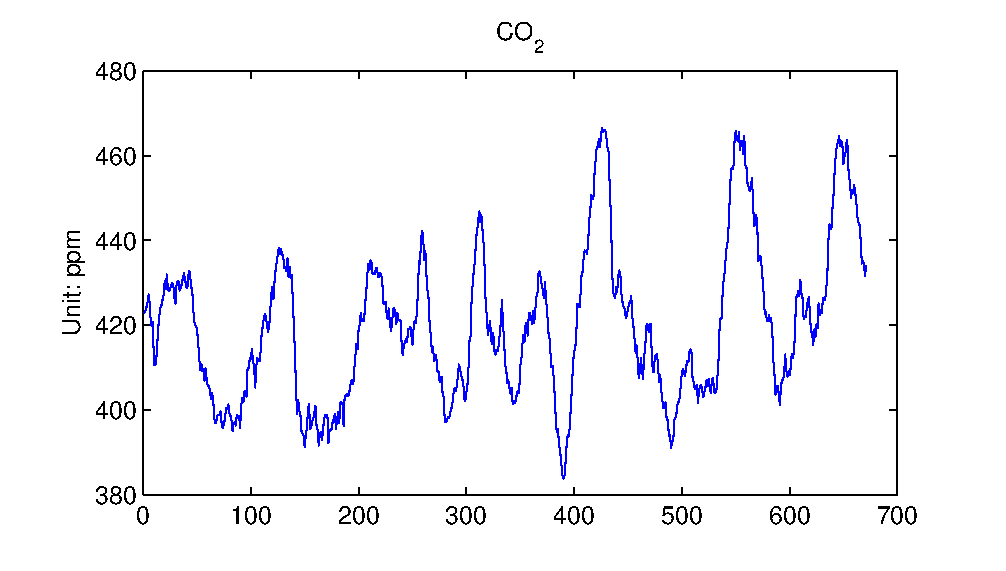
\includegraphics[width=\textwidth]{./fig/co2.eps}
                \caption{$CO_{2}$}
  \end{subfigure}
  \begin{subfigure}{0.32\textwidth}
                \centering
    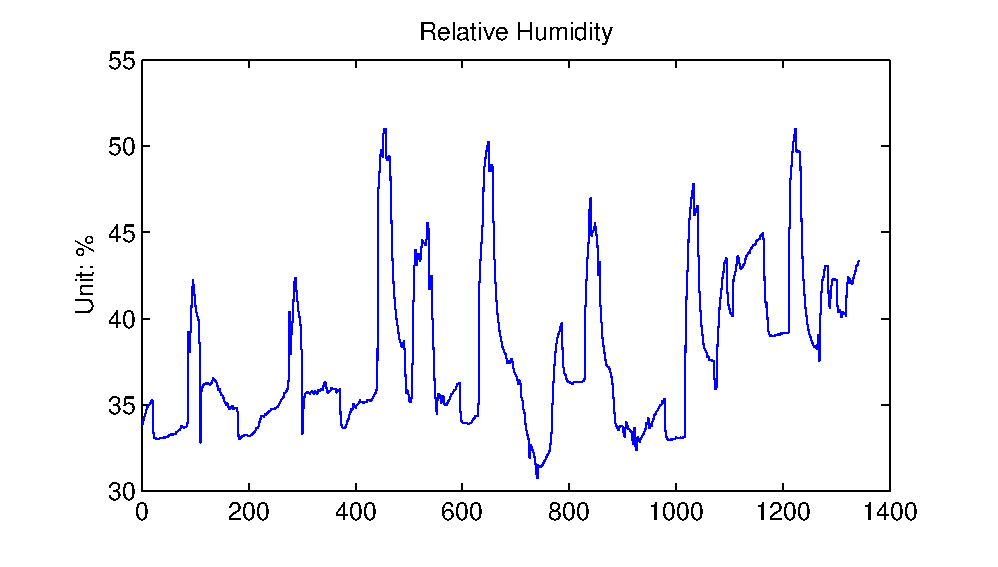
\includegraphics[width=\textwidth]{./fig/rh.eps}
                \caption{Humidity}
  \end{subfigure}
  \begin{subfigure}{0.32\textwidth}
                \centering
    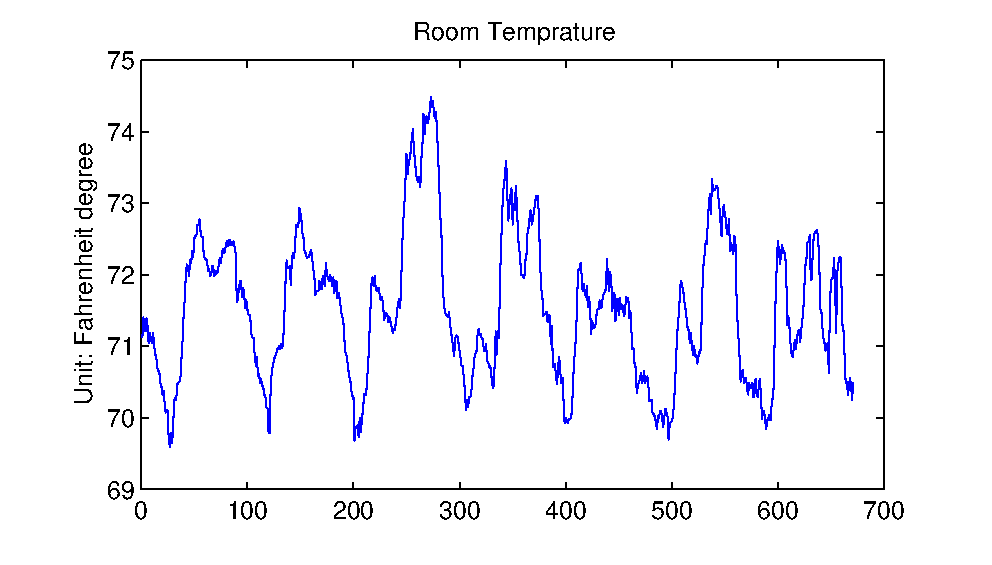
\includegraphics[width=\textwidth]{./fig/rmt.eps}
                \caption{Room Temperature}
  \end{subfigure}
  %row2
  \begin{subfigure}{0.32\textwidth}
                \centering
    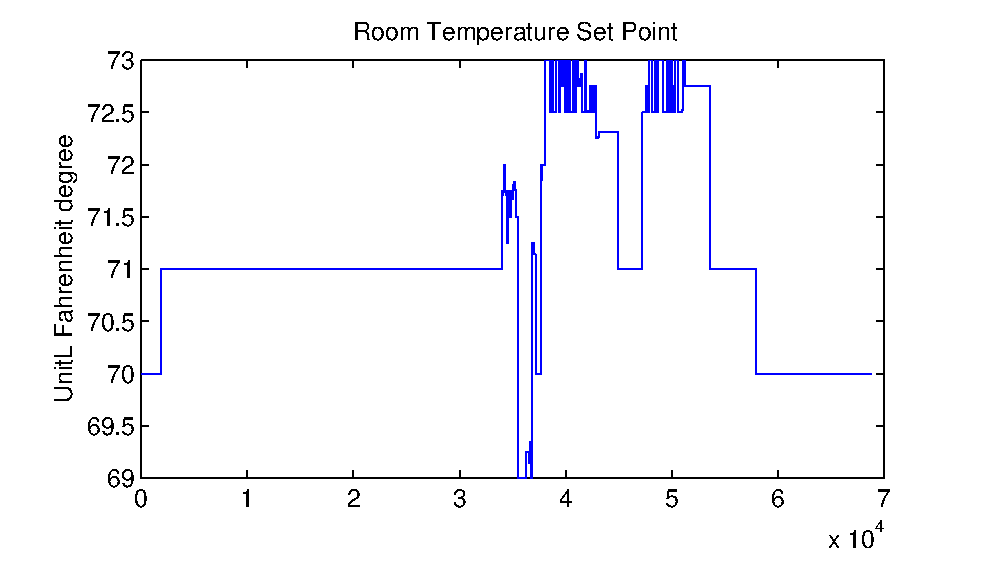
\includegraphics[width=\textwidth]{./fig/stpt.eps}
                \caption{Room Temperature Set Point}
  \end{subfigure}
  \begin{subfigure}{0.32\textwidth}
                \centering
    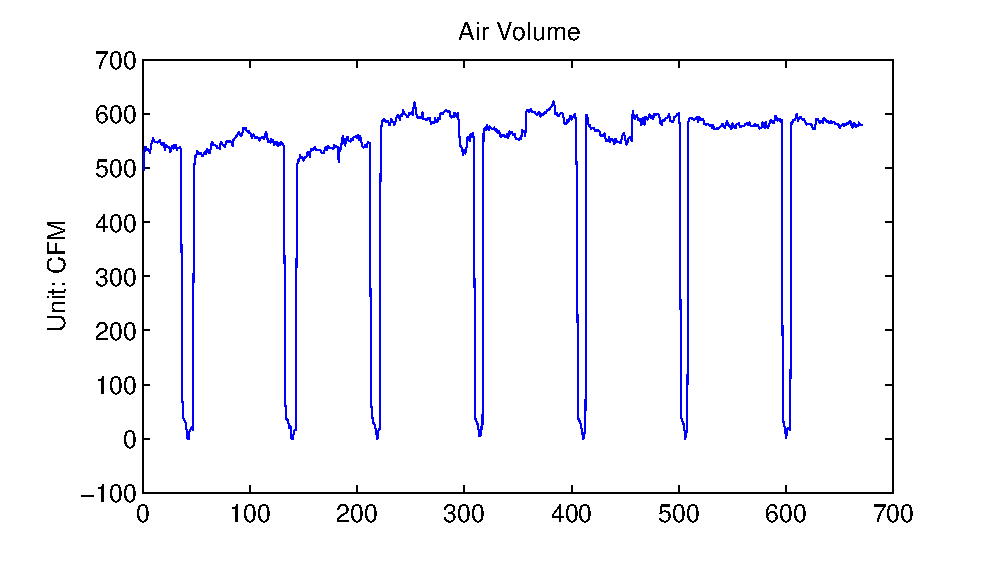
\includegraphics[width=\textwidth]{./fig/vav.eps}
                \caption{VAV Air Volume}
  \end{subfigure}
  \begin{subfigure}{0.32\textwidth}
                \centering
    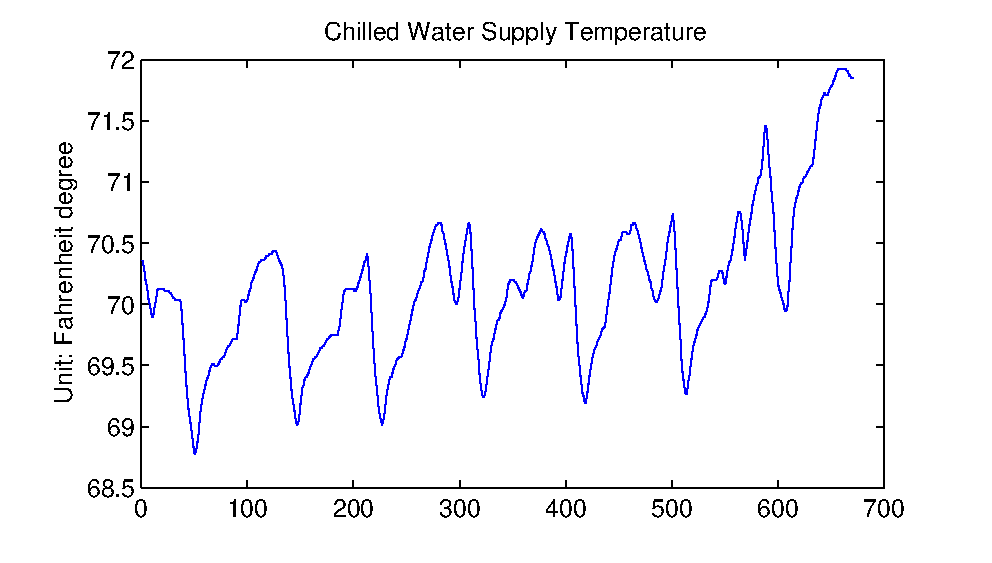
\includegraphics[width=\textwidth]{./fig/cwt.eps}
                \caption{Chilled Water Supply Temperature}
  \end{subfigure}
\caption{Different types of sensors occupy different amplitude bins in the time domain with different short term dynamics.}
\label{fig:example}
\end{figure*}

\subsection{Data Features}
Raw sensor time series\footnote{In this paper, we use the term ``trace'' and ``time series'' \textit{interchangeably}.} usually contain millions of readings which are too many to be useful for type classification. We need to distil the information embedded in the reading patterns.
A signal in the time domain trends the sensor reading and different types of sensor generally occupy distinct amplitude bins, as demonstrated in Figure~\ref{fig:example}. 
We characterize the distribution of a signal in the time domain with standard statistical features, such as the 50th percentile value (also known as the median) as discriminators. 
Table~\ref{table:fd} summarizes the statistical features we used to represent each stream. 


\begin{table}[h]
\centering
\begin{tabular}{r|l|l}
\hline
Category                   & Statistical Function & \multicolumn{1}{l}{Acronym} \\ \hline\hline
\multirow{2}{*}{Extreme}   & Minimum                 & min                          \\ \cline{3-3} 
                           & Maximum                 & max                          \\ \hline
\multirow{2}{*}{Average}   & Median                  & emd                          \\ \cline{3-3} 
                           & Root Mean Square        & rms                          \\ \hline
\multirow{2}{*}{Quartiles} & 1st and 3rd Quartiles   & 1q, 3q                       \\ \cline{3-3} 
                           & Inter-quartile range    & iqr                          \\ \hline
\multirow{3}{*}{Moments}   & Variance                & var                          \\ \cline{3-3} 
                           & Skewness                & skew                         \\ \cline{3-3} 
                           & Kurtosis                & kurt                         \\ \hline
Shape                      & Linear Regression Slope & slope                        \\ \hline
\end{tabular}
\caption{Statistical features extracted in window level for each time series data.}
\label{table:fd}
\end{table}


We segment each sensor readings into an hour-long windows and extract the above features within each window. 
However, computing features over these short time windows will produce too much information as well as noise; too many feature variables typically degrades classifier performance.
To succinctly summarize the dynamics of sensor traces, we compute the statistics of the accumulated features from windowed slices as the final feature set. 
We construct our feature vector as follows: first, each sensor trace is segmented into N non-overlapping one-hour long windows. Second, within each time window, we compute the statistics as in the above table for the trace, producing a vector of each statistical feature after the window slides over the entire trace, such as 
$MIN = \{min^{1}, min^{2}, ..., min^{N}\}$, where N is the number of time windows. Each vector (such as this $MIN$) reflects short term changes but not all the intermediate values are useful for classification. 
Finally, we compute a statistical summary of these vectors. For each vector we compute the minimum, maximum, median and variance, resulting in a feature vector containing 44 variables:
\begin{displaymath}
\begin{split}
F = \{min(MIN), max(MIN), median(MIN), var(MIN),\\
...\\
min(SLOPE), max(SLOPE), median(SLOPE), var(SLOPE)\}
\end{split}
\end{displaymath}
$F$ is the data feature vector for each sensor trace used in our study.


\subsection{Name Features}
The sensor point names are short text strings with several concatenated abbreviations, as shown in our motivating example in Table~\ref{table:ex}. 
To represent the primitive point names as feature vectors for classifier training, we first convert all point names to lower cases and trim out the numerical characters in each point name, resulting in a series of words, e.g., \texttt{Zone Temp 2 RMI204} becomes \texttt{\{zone, temp, rmi\}}. 
To capture possible variants of abbreviations in point names, e.g., ``tmp'' and ``temp'' for temperature, we adopt $k$-mers \cite{leslie2004mismatch} as our features. 
The term $k$-mer refers to all the possible substrings of length $k$, which are contained in a string. This feature is popularly used in protein and gene sequence analysis in bioinformatics, and it helps measure sequence similarity without requiring alignment. 

In our case, we limit the k-mers computation only within a word boundary.
In general, having a too small $k$ will increase the chance for all the k-mers to overlap, making all the points less differentiable.
Therefore, we compute all k-mers of length 3 and 4 for each point name.
For example, \texttt{\{zone, temp, rmi\}} will yield a set of k-mers \texttt{\{zon, one, tem, emp, rmi\}} with $k$=3.
A dictionary of k-mers is constructed with all the k-mers generated from each point name. 
Each point name is converted into a feature vector based on the frequency of k-mers in it. 
For example, a set of k-mers \texttt{\{zon, tem, emp, zon\}} will be transformed to a vector
\texttt{(2,0,1,1,0)} with the dictionary \texttt{\{zon, one, tem, emp, rmi\}}, meaning \texttt{zon} occurs twice, \texttt{one} doesn't appear, and so forth. 
This feature representation of point names will be used for examining classification performance.

\subsection{Transferability}
Now with the two different types of features explained, we examine how well both can perform in classifying sensor types when applied across buildings, i.e., learning a classifier based on the features from building A and testing it on building B. 
Intuitively, data features should be more generalizable than point names with respect to differentiating points by types. 
This is because in general a certain type of sensors will share commonality in reading amplitude and trend, such as diurnal patterns. 
For example, temperature readings in a building will be between 60-70 degree with rises in the morning and falls at night.
In contrast, point name features might not transfer well due to various naming conventions across buildings as shown in Table~\ref{table:ex}.
Although k-mers can enlarge the size of term dictionary in a building to increase the chance of covering more terms in other buildings, such a technique still cannot fundamentally compensate for the difference in naming conventions.

\begin{table}[h]
\centering
\begin{tabular}{l|c|c}
\hline
                & Data Feature & Name Feature \\ \hline
A-\textgreater B & 0.778       & 0.341       \\
B-\textgreater A & 0.612       & 0.328       \\ \hline
\end{tabular}
\caption{Type classification accuracy between two buildings with different sets of features.}
\label{table:clf}
\end{table}


To empirically examine how well each type of feature transfers, we perform type classification across buildings with both features in separate. With either set of features from building A, we train a linear SVM and apply it to building B on the same type of feature, or vice versa. Table~\ref{table:clf} summarizes the results.
We see that data features do transfer better than name features as expected, but the results from data features still contain significant errors making them far from being usable. 
The question remains how to better leverage these two sources of information from one building and transfer them to another.
We will discuss the idea of transfer learning in next section.



\section{Related Work}
To the best of our knowledge, we are the first to approach the problem of sensor type classification leveraging knowledge across buildings.

Bhattarcharya et al~\cite{arka} exploit a programming language based solution, 
where they derive a set of regular expressions from a handful of labeled examples 
to normalize the point name of sensors. 
This approach assumes a consistent format for all point names, which is not the case in practice, as shown in Table~\ref{table:ex}. 
Schumann et al~\cite{ibm} develop a probabilistic framework to classify sensor types 
based on the similarity of a raw point name to the entries in a manually constructed dictionary. 
However, the performance of this method is limited by the coverage and diversity of entries listed in the dictionary, and the dictionary size becomes intractable when there exist a lot of variations of the same type, or conflicting definitions of a dictionary entry in different buildings.
Hong et al~\cite{cikm} formulate an active learning based approach to iteratively 
acquire human labels for the building and propogate pseudo labels among points.
However, none of these prior work addresses the scalability issue of metadata 
normalization nor leverages the knowledge from already labeled buildings.

There are several categories of tranfer learning as comprehensively surveyed in~\cite{transfer1}. We only briefly summarizes the differences. Inductive transfer learning~\cite{transfer2} assumes the set of class labels in the target domain is different from the source domain, no matter the feature spaces are the same or not. Multi-task learning~\cite{multitask} has a similar setting, but inductive transfer learning only aims at achieving high performance in the target task by transferring knowledge from the source task while multitask learning tries to learn the target and source task simultaneously. Transductive transfer learning~\cite{transfer3} assumes the source and the target have the same set of labels no matter the feature spaces are the same or not; our problem setting falls into this category. There has also been active research on how to construct an ensemble of classifiers and some assign local weights locally~\cite{ensem1,ensem2}, however, these local weights are decided only based on the training data.
Instance-based local weighting~\cite{weight1,weight2,weight3} has also been well studied, but these work assumed that the training and testing distributions differ only in $p(x)$ but not in $p(y|x)$.

%Timeseries Representation~\cite{sax,shapelet1,shapelet2}

\section{Transfer Learning}
In this work, we adopt a transfer learning based approach~\cite{lwe} to classify sensor types 
in one building and use the learned model to label sensors in another building.
%for a building with the knowledge from another labeled building. 
The approach presented in~\cite{lwe} uses a suite of base classifiers and leverges the consistency between classifier and cluster structure 
to weigh the results of each classifier.
%as the weight for each base classifier. 
We make several changes to the original algorithm to address the specific challenges we face: 
1) both data features and name features are used by our classifier: an 
ensemble of base learners are constructed with data features and applied to the target building, while the 
cluster structure on the name features in the target building guides the decision process about how to weigh each classifier; %which base classifier should be weighed
%more heavily; %should gain more weights in predictions; 
2) we customize the weight estimation algorithm to improve its performance in our setting; %domain and make it more effecitve; 
and 3) to handle variations in point names, we use a non-parametric Bayesian approach to identify cluster structure.

\subsection{Feature Representation}\label{feature}
Two common attributes of the sensor points in a building are the actual data readings and the text string-based point names. Both play an important role for differentiating sensor types.
In this section, we elaborate the construction of two different sets of feature vectors, i.e., data features and name features.

\begin{figure*}[ht!]
\centering
  \begin{subfigure}{0.32\textwidth}
                \centering
    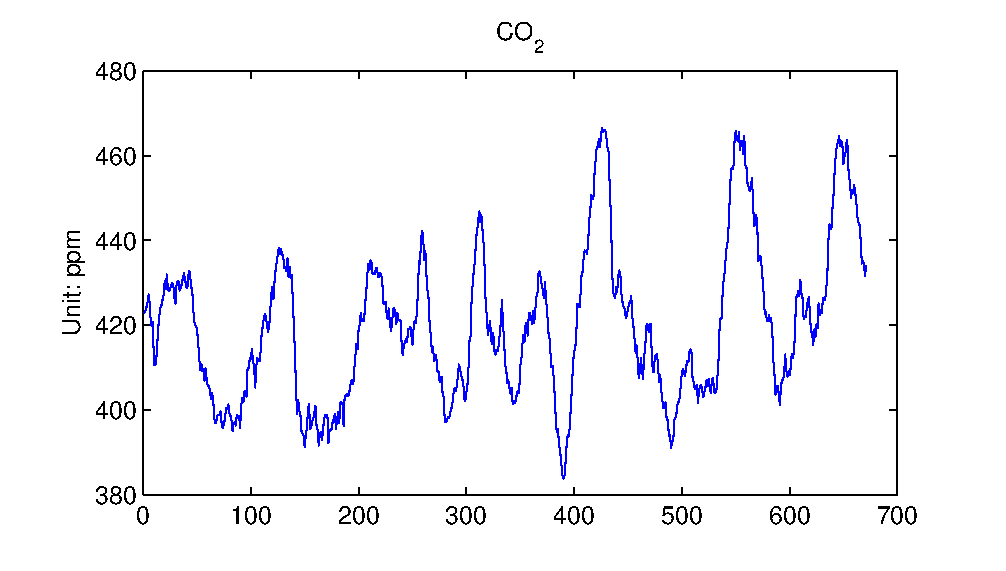
\includegraphics[width=\textwidth]{./fig/co2.eps}
                \caption{$CO_{2}$}
  \end{subfigure}
  \begin{subfigure}{0.32\textwidth}
                \centering
    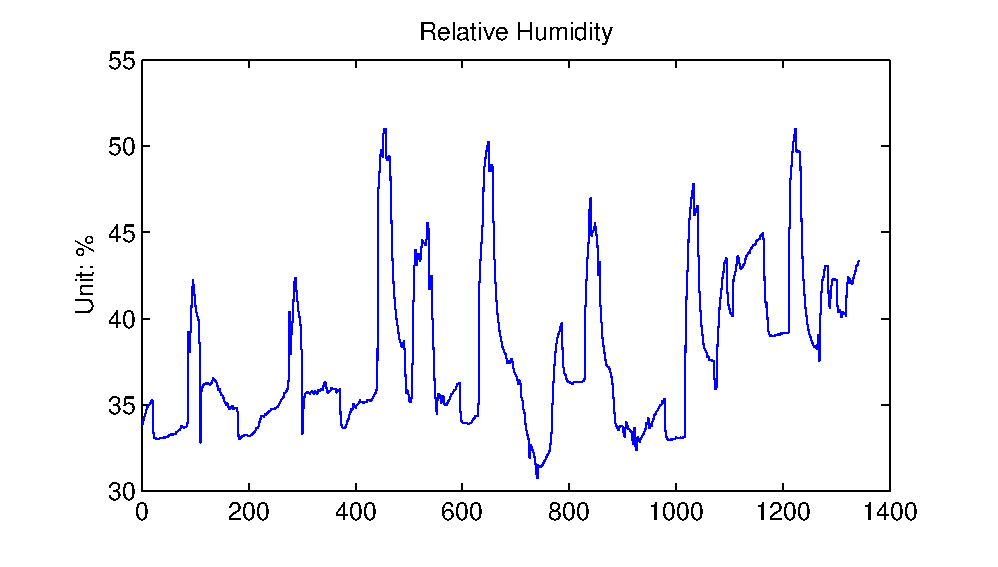
\includegraphics[width=\textwidth]{./fig/rh.eps}
                \caption{Humidity}
  \end{subfigure}
  \begin{subfigure}{0.32\textwidth}
                \centering
    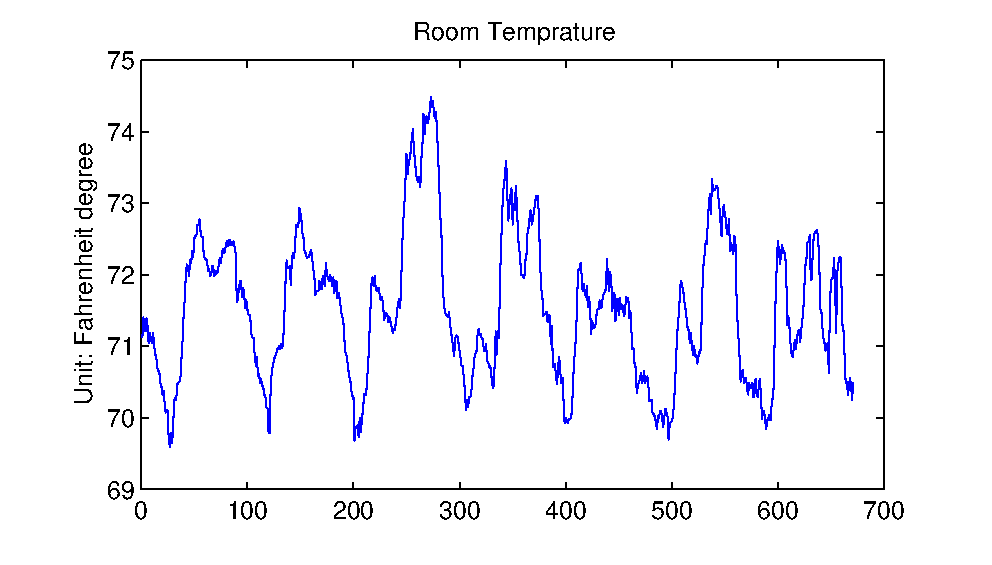
\includegraphics[width=\textwidth]{./fig/rmt.eps}
                \caption{Room Temperature}
  \end{subfigure}
  %row2
  \begin{subfigure}{0.32\textwidth}
                \centering
    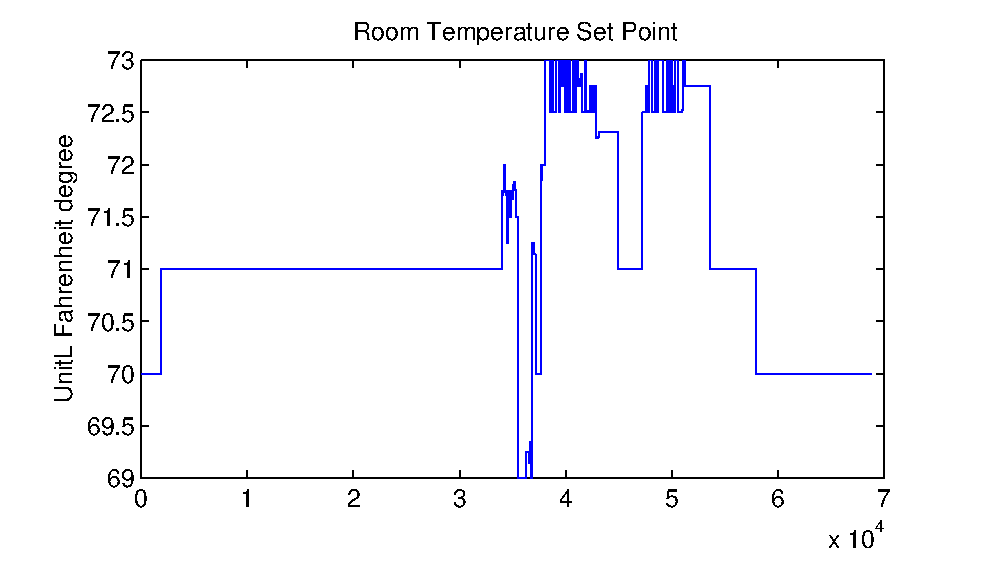
\includegraphics[width=\textwidth]{./fig/stpt.eps}
                \caption{Room Temperature Set Point}
  \end{subfigure}
  \begin{subfigure}{0.32\textwidth}
                \centering
    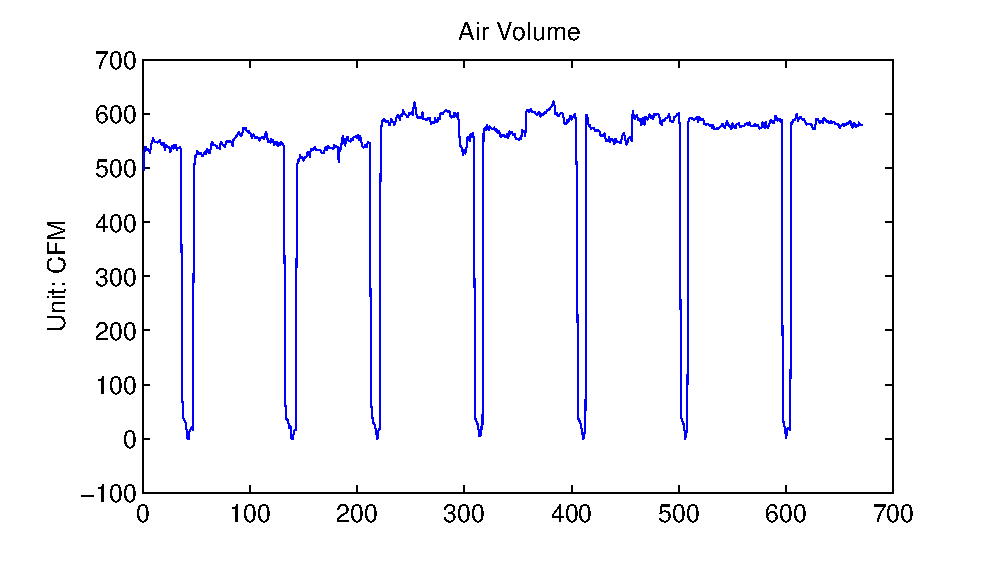
\includegraphics[width=\textwidth]{./fig/vav.eps}
                \caption{VAV Air Volume}
  \end{subfigure}
  \begin{subfigure}{0.32\textwidth}
                \centering
    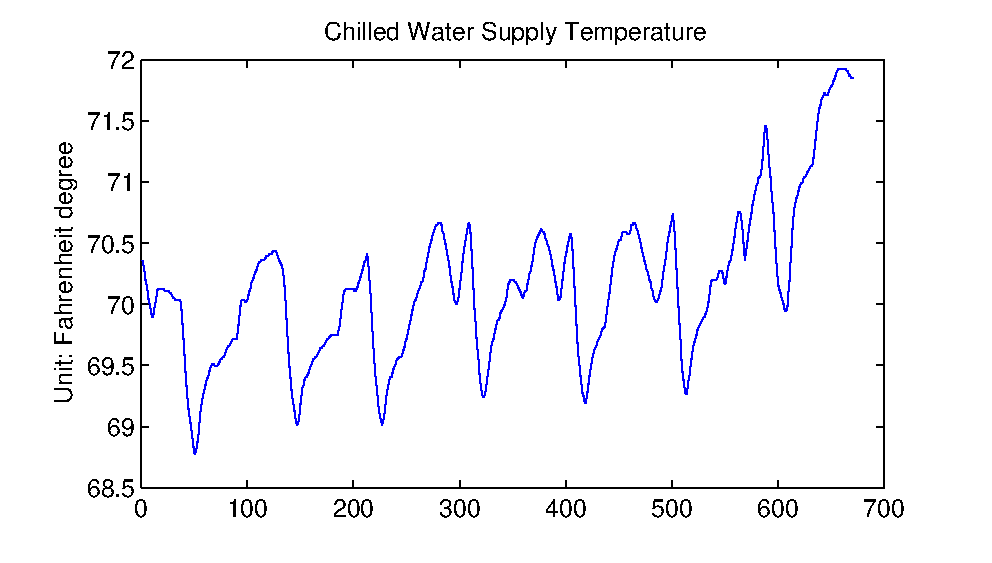
\includegraphics[width=\textwidth]{./fig/cwt.eps}
                \caption{Chilled Water Supply Temperature}
  \end{subfigure}
\caption{Different types of sensors occupy different amplitude bins in the time domain with different short term dynamics.}
\label{fig:example}
\end{figure*}

\subsubsection{Data Features}
A signal\footnote{In this paper, we use the term ``signal'', ``trace'' and ``time series'' \textit{interchangeably}.} in the time domain is a trend of sensor reading. 
Different types of sensor generally have different amplitudes that can be separated and binned,  
%occupy distinct amplitude bins, 
as demonstrated in Figure~\ref{fig:example}. 
Similar to piecewise aggregated approximation (PAA~\cite{paa}) -- where the mean is calculated in a fixed-length window -- 
we compress the signal by computing a set of summary statistics over fixed-length windows. 
%we compress a signal in a time window with summary statistics that characterize the behavior of the signal in that window.
%characterize a windowed signal in the time domain with 
%standard statistical features which are summarized in .
Table~\ref{table:fd} shows a summary of the statistics we calculate. %we use to vectorize a time window.


\begin{table}[h]
\centering
\begin{tabular}{r|l|l}
\hline
Category                   & Statistical Function & \multicolumn{1}{l}{Acronym} \\ \hline\hline
\multirow{2}{*}{Extreme}   & Minimum                 & min                          \\ \cline{3-3} 
                           & Maximum                 & max                          \\ \hline
\multirow{2}{*}{Average}   & Median                  & emd                          \\ \cline{3-3} 
                           & Root Mean Square        & rms                          \\ \hline
\multirow{2}{*}{Quartiles} & 1st and 3rd Quartiles   & 1q, 3q                       \\ \cline{3-3} 
                           & Inter-quartile range    & iqr                          \\ \hline
\multirow{3}{*}{Moments}   & Variance                & var                          \\ \cline{3-3} 
                           & Skewness                & skew                         \\ \cline{3-3} 
                           & Kurtosis                & kurt                         \\ \hline
Shape                      & Linear Regression Slope & slope                        \\ \hline
\end{tabular}
\caption{Statistical features extracted in window level for each time series data.}
\label{table:fd}
\end{table}

Our feature extraction process consists of three steps.
First, each sensor trace is segmented into N non-overlapping hour-long windows. Second, within each time window, we compute the statistics shown above. 
%This produces a vector where each component is a a %statistic over the window. %slides over the entire trace, such as 
For example, the $MIN$ vector is computed as follows: 
$MIN = \{min^{1}, min^{2}, ..., min^{N}\}$, where N is the number of time windows. We compute a similar vector for each statistic show in the table.
%Each vector, reflects short term changes that are useful for classification. 
Third, we compute a statistical summary of these vectors. For each vector we compute the minimum, maximum, median and variance, resulting in a feature 
vector containing 44 variables:
\begin{displaymath}
\begin{split}
F = \{min(MIN), max(MIN), \\ 
median(MIN), var(MIN),\\
...\\
min(SLOPE), max(SLOPE), \\
median(SLOPE), var(SLOPE)\}
\end{split}
\end{displaymath}
$F$ is the data feature vector for each sensor trace used in our study.


%First, 
%we segment each timeseries into hour-long windows and calculate the given statistics. %the above features within each window. 
%Then, we
%Since computing over features these short time windows will produce too much information as well as noise; 
%therefore we compute the statistics of the accumulated features from windowed slices as the final feature set. 

\subsubsection{Name Features}
Sensor point names are short text strings with several concatenated abbreviations, as shown in Table~\ref{table:ex}. 
To vectorize a point name, we convert all alpha characters to lower case and trim out numerical characters. 
For example, \texttt{Zone Temp 2 RMI204} becomes \texttt{\{zone, temp, rmi\}}. 
%To capture possible variants of abbreviations in point names, e.g., ``tmp'' and ``temp'' for temperature, we adopt $k$-mers \cite{leslie2004mismatch} as our features. 
We use $k$-mers \cite{leslie2004mismatch} to capture variations in type abbreviations, e.g., ``tmp'' and ``temp'' for temperature.
The term $k$-mer refers to all the possible substrings of length $k$, which are contained in a string. This feature is often used in protein and gene sequence analysis and 
it helps measure sequence similarity without requiring alignment. 

We limit the k-mers computation within a word boundary.
In general, having too small a value for $k$ will increase the chance for all the k-mers to overlap, making points less differentiable.
Therefore, we compute all k-mers of length 3 and 4 for each point name.
For example, \texttt{\{zone, temp, rmi\}} yields a set of k-mers \texttt{\{zon, one, tem, emp, rmi\}} when $k$=3.
A dictionary of k-mers is constructed with all the k-mers generated from each point name. 
Each point name is converted into a feature vector based on the frequency of k-mers in it. 
For example, a set of k-mers \texttt{\{zon, tem, emp, zon\}} will be transformed to a vector
\texttt{(2,0,1,1,0)} with the dictionary \texttt{\{zon, one, tem, emp, rmi\}}, meaning \texttt{zon} occurs twice, \texttt{one} does 
not appear, and so forth. 
This feature representation of point names will be used for examining classification performance.


\subsection{Knowledge Transfer}
%The use of transfer learning is motivated by the fact that people often have one or only a few buildings labeled of which they want to take advantage to aid the labeling of a new buidling.
Transfer learning a useful technique in the building space because the effort it takes to label sensors in a single building is 
high.  We want to leverage the knowledge gained in one building to quickly label another with minimal effort.  
Transfer learning uses well-labeled data from one domain\footnote{A ``domain'' particularly refers to a data set  in this paper.}  
to classify samples in a new, related domain.
We assume we have well-labeled training set examples but do not have any labeled examples from the testing set. 
Such knowledge transfer is only possible when the training domain and the test domain have the same set of class labels. 
Classical supervised learning techniques are not useful for transferring knowledge across domains in this setting because 
%The reason that traditional supervised learning techniques is not successful in transferring knowledge across domains in our case is because 
it requires the training and testing examples to be sampled i.i.d. from the same distribution. This basic requirement does not hold here.

%For example, the classiers can be trained from several relevant domains or built using different learning algorithms on the same domain.
To encapsulate the information from one labeled building and transfer it across buildings, we construct a few classifiers with different 
learning algorithms, using the same set of data features from the source building\footnote{the building we learn from is the ``source'', all others are ``targets''}.   
Each classifier contains a different ``perspective'' for that building, due to the inductive bias of the underlying model. 
We refer to these classifiers as {\it base} models\footnote{We use the term ``model'' and ``classifier'' {\it interchangeably} in this paper.} and combine them for 
classification in the target building.
We will discuss the choice of data features for classifier training in the evaluation.


\subsection{Locally Weighted Ensemble}
Different models can be effective at different regions or structures in the new testing building, and no single model can perform well on all examples. 
Ideally, we want to combine the knowledge in the base models, rather than only using any particular model, to more effectively transfer the knowledge to the new building. 
% A natural choice is model averaging that additively combines the predictions of multiple base learners. 
% However, the existing model averaging methods for traditional supervised learning usually assign global weights to models, which are either uniform (e.g., in Bagging~\cite{bagging}) or proportional to the training accuracy (e.g., in Boosting~\cite{boosting}), or simply relying on a specific model (e.g., single model classification).
% Such global weighting schemes may not perform well in transfer learning because different testing examples may favor predictions from different base models. 
% For example, when the base models carry conflicting concepts at a testing example, the optimal choice would be a model that better represents the distribution underlying the example.
We employ a locally weighted ensemble~\cite{lwe} to weight the predictions from base classifiers. 
The weight is computed per model per example based on the similarity between the model and the local structure of the target example. 
The similarity is measured by comparing neighborhood graphs which we will explain in the next section. 
Such local weighting will favor models whose predicted local structure is close to the true local structure of the target example in the new testing domain. 
Let $x$ be the data feature vector of an example in the new building and $y$ be its predicted class label. Given a set of $k$ base models $M_1, \dots, M_k$ and the new testing set $D_T$ represented in the data feature view, the general Bayesian model averaging rule to estimate the posterior distribution of $y$ is,
\begin{equation}\label{eq_lwe}
p(y|x)=\sum_{i=1}^k p(y|x,D_T,M_i) p(M_i|D_T)
\end{equation}
where $p(y|x,D_T,M_i) = p(y|x,M_i)$ because $x \in D_T$ and $p(y|x,M_i)$ is actually the prediction on $x$ by $M_i$. And $p(M_i|D_T)$ is the probability to choose $M_i$ given the testing set $D_T$. As $x \in D_T$, $p(M_i|D_T)$ equals to $p(M_i|x)$ which is the locally adjusted weight for $M_i$ and Eq.~\ref{eq_lwe} becomes,
\begin{equation}\label{eq_sum}
p(y|x)=\sum_{i=1}^k w_{x}^{M_i} p(y|x, M_i)
\end{equation}
where $w_{x}^{M_i} = p(M_i|x)$ and intuitively, a model $M_i$ should have higher weights for $x$ if $M_i$ predicts a similar local structure of $x$ to the true one.
We will next explain how the weight is calculated per example.

\subsection{Graph-based Weight Estimation}\label{sec:gwe}
% If $p(y|x)$ is known, we can estimate the weights $w_{x}^{M_i}$ for each model by minimizing the square error between its prediction and the ground truth. 
% However, in practice the truth value of $p(y|x)$ for a new building is not available a priori . 
% The main task becomes to properly define the similarity between classifier's predicted structure and the true structure. 
We quickly summarize the graph-based weight estimation in~\cite{lwe} and describe our two adjustments which are customized for our problem.
Following the assumption~\cite{cluster} that $p(y|x)$ is not expected to change much in a dense area where $p(x)$ is high, 
% which means the decision boundary probably exists in areas with smaller $p(x)$.
~\cite{lwe} performs clustering on the new testing set and assume the boundaries between clusters represent areas where $p(x)$ is small.
If the clustering boundary for the region where $x$ locates agrees with the decision boundary of $M_i$, 
% we assume that $p(y|x,M_i)$ is similar to the true $p(y|x)$ around $x$, which means 
a larger weight is assigned to $M_i$ at $x$.
In other words, if the predictions of $M_i$ on the area surrounding $x$ have higher consistency with the clustering results, $M_i$ would have a larger weight at $x$. 

Based these observations, the weight is estimated with a graph-based algorithm.
To compute the $w_{x}^{M_i}$ for $M_i$ at example $x$, we construct two neighorhood graphs: 
$G_M = (V, E_M)$ and $G_C = (V, E_C)$, for classification and clustering respectively, 
where each vertex is an example and $V = D_T$. In $G_M$, an edge exists between two vertices (denoting the two examples are ``neighbors'') if and only if $M_i$ predicts the same label for these two examples. Likewise, in $G_C$, an edge exists between two vertices if and only if these two examples reside in the same cluster.
If the neighbors of $x$ on both graphs significant overlap, then $M_i$ will be assigned a larger weight.
So the weight $w_{x}^{M_i}$ for $M_i$ at $x$ is proportional to the similarity of the two graphs:
\begin{equation}\label{eq_sim}
w_{x}^{M_i} \propto s(G_M, G_C|x) = \frac {|V_M \cap V_C|} {|V_M \cup V_C|}
\end{equation}
where $V_M$ ($V_C$) is the set of neighbors of $x$ on graph $G_M$ ($G_C$), |$\cdot$| is the cardinality of a set, and $s(G_M, G_C|x)$ is the similarity between two graphs. 
Figure~\ref{fig:graph} illustrates an example of neighborhood graphs for an example $x$ (in grey circle): model 1 has a similarity of 0.75 while model 2 has 0.5.

\begin{figure}[h]
\centering
    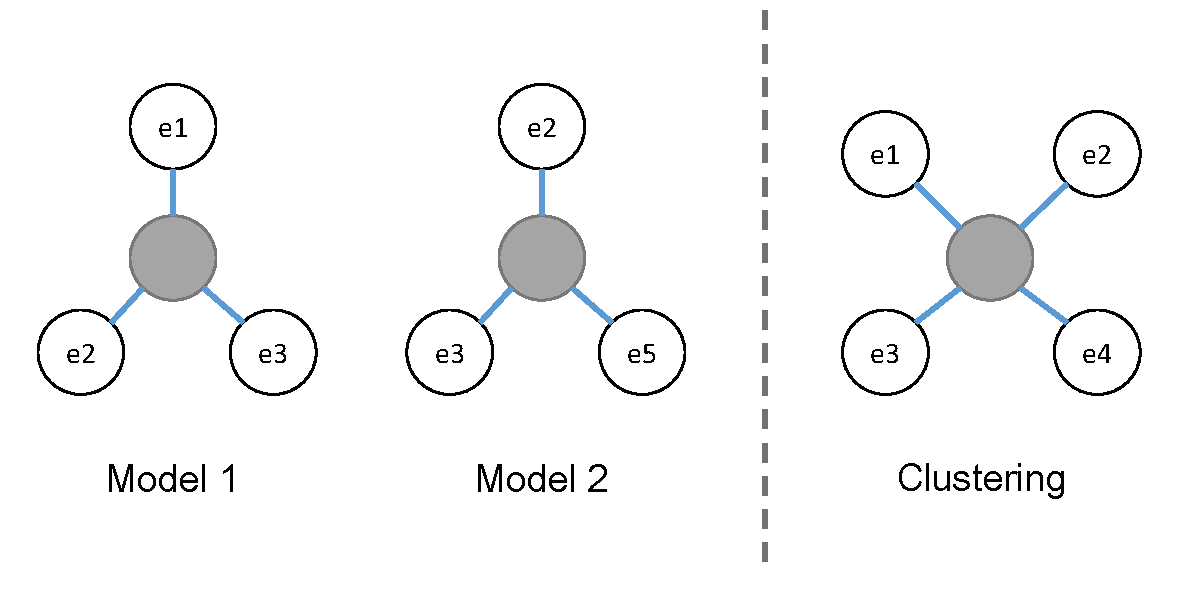
\includegraphics[width=0.4\textwidth]{./fig/lwe_graph}
\caption{An example of local neighborhood graphs of $x$ (in grey circle).}
\label{fig:graph}
\end{figure}

With Eq.~\ref{eq_sim} defined, the weight for each $M_i$ is calculated by normalizing among all similarity scores:
\begin{equation}\label{eq_norm}
w_{x}^{M_i} = \frac {s(G_{M_i}, G_C|x)} {\sum_{i=1}^k s(G_{M_i}, G_C|x)}
\end{equation}
And the final prediction for $x$ is simply $\hat y = argmax_y \enspace p(y|x)$ as $p(y|x)$ is defined in Eq.~\ref{eq_sum}.

\subsubsection{Distance-based Adjustment}
We notice in some cases the original similarity definition can be problematic. Consider the case as shown in Figure~\ref{graph_dist}, there are two neighbors on both of the graphs for the two models and the distance between vertices are marked on the edge. Since the original similarity definition only considers the number of neighbors, both models will be assigned the same weight of 0.5 in this case while obviously model 1 ought to have a higher weight because the neighbors on
the left graph are closer to the target example.
To fix the issue, we include the distance between examples into consideration, the adjusted similarity is:
\begin{equation}\label{d_sim}
s^\ast(G_M, G_C|x) = 1 - \frac {\sum d_{V_I}/|V_I|} {\sum d_{V_U}/|V_U|}
\end{equation}
where $V_I = V_M \cap V_C$, $V_U = V_M \cup V_C$, and $\sum d_{V_I}$ is the sum of distance between $x$ to its neighbors in $V_I$ (likewise for $\sum d_{V_U}$).

\begin{figure}[h]
\centering
    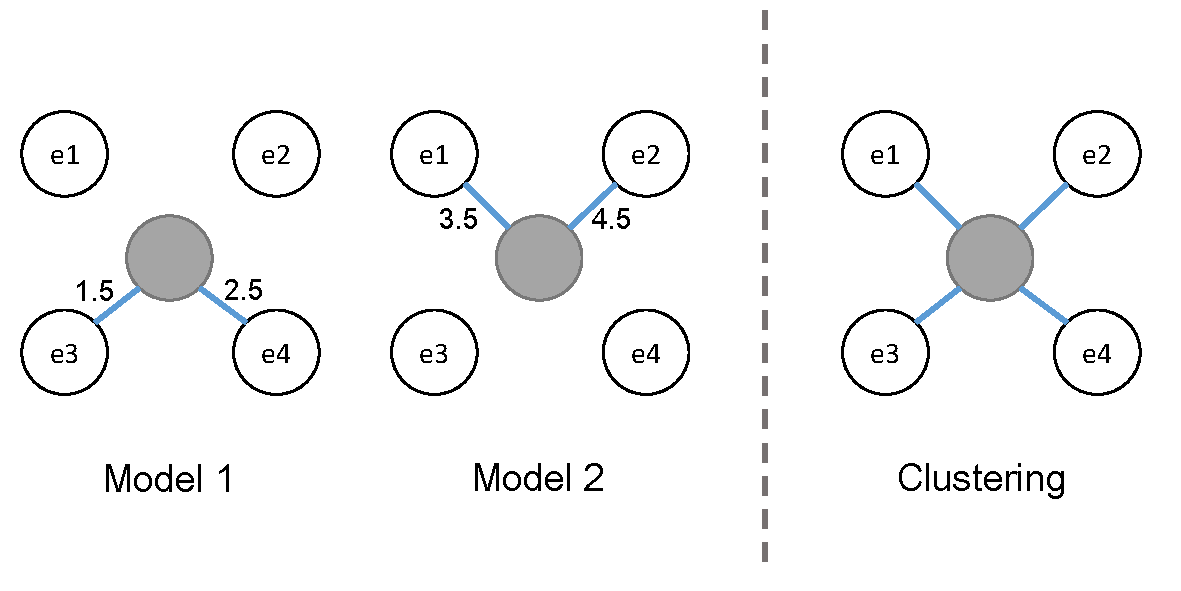
\includegraphics[width=0.4\textwidth]{./fig/lwe_d_graph}
\caption{An example of local neighborhood graphs of $x$ with distance into consideration.}
\label{graph_dist}
\end{figure}

\subsubsection{Thresholding-based Adjustment}
The use of weighted average decision for $x$ among base classifiers is reasonable when at least some of these classifiers perform well on $x$. However, the similarity $s(G_{M_i}, G_C|x)$ for $M_i$ is expected to be small when the predictions of $M_i$ around $x$ conflict with its true local structure. 
In such a case, still adopting the decision from the classifier might not be a reasonable choice. 
Since $s(G_{M_i}, G_C|x)$ reflects the consistency between classifier predictions and cluster structure, we use the average similarity score over all $M_i$ on $x$ as a discriminator to limit the usage of these base classifiers.
As an adjustment before the normalization of similarity scores, we check the average similarity score with,
\begin{equation}\label{ave_sim}
 \bar s_x = \frac {1}{k}\sum_{i=1}^k s(G_{M_i}, G_C|x)
\end{equation}
We will continue with the ensemble prediction only if $\bar s_x$ is larger than a threshold $\delta$, and we will discuss the choice of $\delta$ in the evaluation section.


\subsection{Clustering with Non-parametric Bayesian}
\label{sec_clustering}
In our transfer learning based approach, data density $p(x)$ is exploited via its latent clustering structure. We choose Gaussian Mixture Model (GMM) \cite{zivkovic2004improved}, a partitional clustering algorithm, to perform the clustering.

In GMM, the cluster label for every instance is treated as a latent variable, which is drawn from a multinomial distribution $p(c)$, i.e., $p(c)\propto\alpha_c$, where $\forall c, \alpha_c\ge0$ and $\sum_c\alpha_c=1$. In any given cluster $c$, the conditional data likelihood of an instance $x$ is specified by a multivariate Gaussian distribution. To reduce the number of parameters to estimate, we choose the isotropic Gaussian in our solution,
\begin{equation}
p(x|c)=(2\pi\sigma^2)^{-d/2}\exp{-\frac{(x-\mu_c)^\mt (x-\mu_c)}{2\sigma^2}}
\end{equation}
where the variance $\sigma^2$ is shared by all the clusters. $\{\alpha_c, \mu_c\}^k_{c=1}$ and $\sigma$ are considered as model parameters in GMM.

However, in GMM, we need to manually specify the number of clusters for a given input data set; and the clustering result of GMM is very sensitive to such setting. More importantly, in our study, usually there is more than one pattern in the point names even for the same type of sensors; therefore we cannot assume one class has only one cluster. It is impossible for us to predefine those optimal cluster sizes. To make clustering feasible on the new building, we appeal to a non-parameter Bayesian solution: we assume the model parameters $(\alpha, \mu)$ in each cluster are also random variables, which are drawn from a Dirichlet Process prior \cite{dp}.

A Dirichlet Process $DP(G_0, \eta)$ with a base distribution $G_0$ and a scaling parameter $\eta$ is a distribution over distributions~\cite{dp}. The base distribution $G_0$ specifies the prior distribution of model parameters, e.g., mean parameter $\mu$ in each cluster, and the scaling parameter $\eta$ specifies the concentration of samples drawn from the DP, e.g., cluster proportion $p(c)$. An important property of the DP is that though the draws from a DP have countably infinite size, they are discrete with probability one, which leads to a probability distribution on partitions of the data. The number of unique draws, i.e., the number of clusters, varies with respect to the data and therefore is random, instead of being pre-specified.

As a result, with the introduced $DP(G_{0}, \eta)$ prior, data density in a given collection of instances can be expressed using a stick-breaking representation
\cite{sethuraman1994constructive}:
\begin{equation}\label{eq_dp_density}
p(x)=\sum_{c=1}^\infty \alpha_c \mathcal{N}(x|\mu_c,\sigma)p(\mu_c|G_0)
\end{equation}
where $\alpha={\alpha}_{c=1}^\infty\sim Stick(\eta)$ represents the proportion of clusters in the whole collection. The stick-breaking process $Stick(\eta)$ for the cluster proportion parameter $\alpha$ is defined as: $\alpha'_c\sim Beta(1, \eta), \alpha_c=\alpha'_c\prod_{i=1}^{c-1}(1-\alpha'_i)$. Since the variance $\sigma^2$ is fixed in all clusters, we use a conjugate prior for $\mu$ in $G_0$, i.e., for $\forall c, \mu_{ci}\sim \mathcal{N}(a,b)$, with the assumption that each dimension in $\mu_c$ is independently drawn from a univariate Gaussian. This will greatly simplify the later on inference procedure.

Because the data density distribution defined in Eq~\eqref{eq_dp_density} only has finite support at the points of $\{\alpha_c, \mu_c\}^k_{c=1}$, we can calculate the posterior distribution of latent cluster labels in each unlabeled instance to discover the clustering structure. Following the sampling scheme proposed in \cite{neal2000markov}, we appeal to a Gibbs sampling method to infer the posterior of cluster membership. Detailed specifications of this sampling algorithm can be found in \cite{neal2000markov}.


{\bf Putting it all together:} Algorithm~\ref{algo} summarizes our transfer learning algorithm for the sensor type classification across buildings. We start from training a few base classifiers with the data features and labels of examples in a source building. We also generate clusters with DP on the name features of examples in the target building. For each example $x$ in the target building, we measure the local similarity score for each base classifier. If the average similarity is significant enough, we compute the weight for each classifier at $x$ by normalizing the similarity score. Finally we calculate the weighted sum of predictions from all base classifier and obtain the label $y$ for $x$.

\begin{algorithm}[ht]
 \caption{Transfer Learning for Sensor Type Classification}
 \label{algo}
 %\SetAlgoLined
 {\bf Input}: Data features of the source building $\mathcal{D_S}=\{x^D_1,x^D_2,\dots,x^D_n\}$ and their labels $\mathcal{Y_S}=\{y_1,y_2,\dots,y_n\}$  data features of the target building $\mathcal{D_T}=\{x^D_1,x^D_2,\dots,x^D_m\}$, and name features of the target building $\mathcal{P_T}=\{x^P_1,x^P_2,\dots,x^P_m\}$\\
 {\bf Output}: predicted labels of the examples in target building $\mathcal{Y}$\\
 Initialize: Generate clusters with $DP(G_{0}, \eta)$ on $\mathcal{P_T}$\\
 Train $k$ classifiers $M_1, \dots, M_k$ based on $\mathcal{D_S}$ and $\mathcal{Y_S}$\;

\For{$x^D$ in $\mathcal{D_T}$}{
Construct neighborhood graphs $G_M$ and $G_C$ for $x^D$ as defined in Section~\ref{sec:gwe} for each $M_i$;\\
Compute the similarity score for each $M_i$ with Eq.~\ref{d_sim};\\
Check the average similarity score $\hat s_x$ over all $M_i$ with Eq.~\ref{ave_sim};\\
If $\hat s_x > \delta$, then use Eq.~\ref{eq_norm} and Eq.~\ref{eq_sum} to predict the label $y$;
}
\end{algorithm}


\section{Evaluation}
To investigate the effectiveness of our method, we evaluate our transfer learning based classification technique on actual data and point names of sensors from three commercial buildings. Extensive experiments demonstrate that our technique is able to accurately classify by type for a considerable portion of examples without human intervention. 
To further demonstrate what the usefulness of the technique, we combine transfer learning with the traditional labeling process to accelerate the learning speed.


\subsection{Taxonomy and Data Collection}
\begin{figure}[t]
\centering
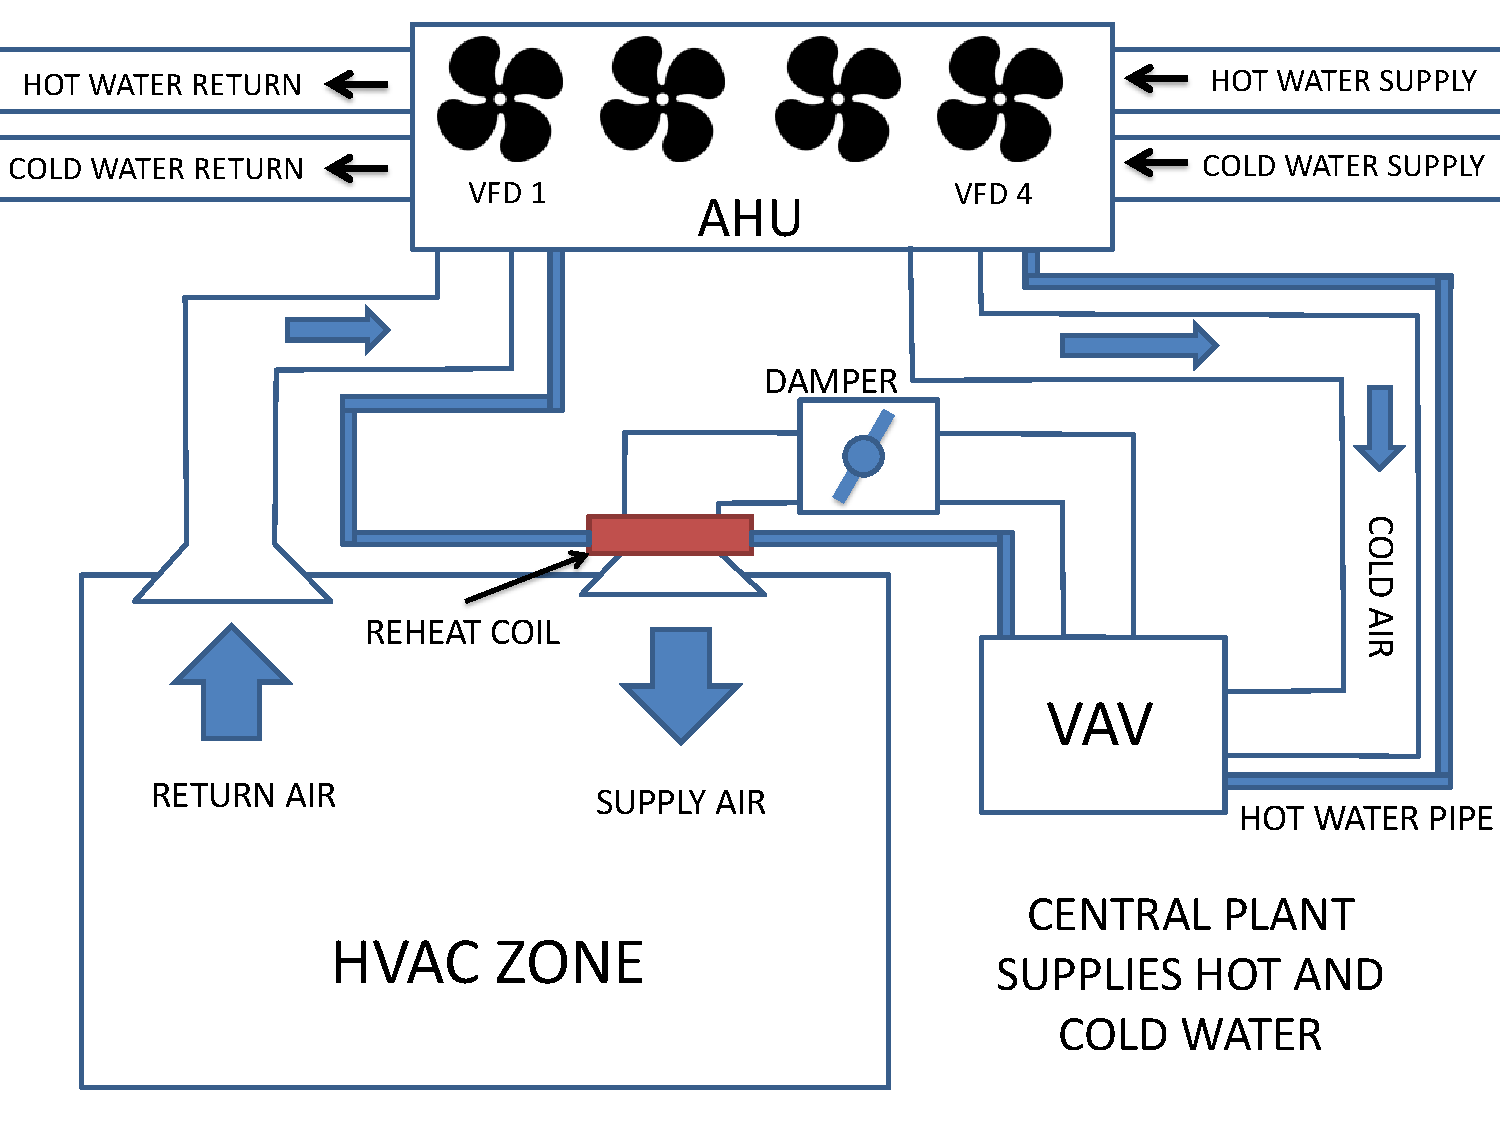
\includegraphics[width=0.38\textwidth]{./fig/hvac}
\caption{A typical HVAC system consisting of an air handler unit (AHU), several variable air volume boxes (VAV), water-based heating/cooling pipes and air circulation ducts. (Figure used with permission from the authors of~\cite{sentinel}.)}
\label{fig:hvac}
\end{figure}

Figure~\ref{fig:hvac} illustrates a typical heating, ventilation, and air conditioning (HVAC) system deployed in modern commercial buildings. 
An HVAC system uses a combination of hot and cold water pipes in conjunction with
air handler units (AHU) to maintain the appropriate thermal environment within the building.
An HVAC system typically consists of several AHUs and each AHU is responsible for a spatial \emph{zone}
in the building. An AHU consists of variable speed drives that supply cold air
(cooled by the supplied cold water) using ducts to VAV boxes distributed throughout the building.
The hot water loop is also connected to these VAV boxes using separate pipes. Each VAV box
controls the amount of air to be let into an HVAC zone using dampers, whose opening angle
can be programmed. A reheat coil, which uses supplied hot water, is used to heat the air to
meet the appropriate HVAC settings for each zone.

Table~\ref{table:num} summarizes all the types of sensors evaluated in our analysis in these three buildings and the number of sensors of each type. 
``Room temperature'' measures the temperature in room. The other temperature measurements for water circulation and air ventilation are illustrated in Figure~\ref{fig:hvac}. 
For setpoints, are grouped together into
one general type. % which includes all set points for every actuator configured in the building.

Our evaluation dataset, which contains both data and point names of sensor streams, is collected from over 2,500 sensors of different types deployed in three commercial buildings. 
We collected a week's worth of data from each building.
Building A is Rice Hall at the University of Virginia, where the sense points report to a database component in a Trane BMS, % anywhere between 
every 10 seconds to 10 minutes.
Both building B and C are from UC Berkeley: B is Sutardja Dai Hall, which contains sensors and equipment from KETI\footnote{\url{http://www.keti.re.kr/}} and Siemens. 
Building C is Soda Hall, which that uses an archaic system by Barrington Controls which is no longer in business. 
Points and sensors in these two buildings transmit data to an sMAP~\cite{smap} archiver periodically between every 5 seconds to 10 minutes.


\begin{table}[t]
\centering
\begin{tabular}{l | l l l}
\hline
& \multicolumn{3}{c}{Building} \\
Type & A & B & C\\
\hline\hline
$CO_{2}$ & 16 & 52 & 0\\
Humidity & 54 & 52 & 0\\
Air Pressure & 142 & 216 & 215\\
Room Temp & 159 & 231 & 208\\
Facility Operation Status & 59 & 72 & 41\\
Facility Control & 0 & 138 & 403\\
Setpoint & 140 & 486 & 229\\
Air Flow Volume & 14 & 172 & 9\\
Damper Position & 0 & 290 & 10\\
Fan Speed & 0 & 25 & 15\\
HW Supply Temp & 27 & 1 & 0\\
HW Return Temp & 15 & 1 & 0\\
CW Supply Temp & 18 & 2 & 11\\
CW Return Temp & 15 & 3 & 10\\
Supply Air Temp & 20 & 17 & 3\\
Return Air Temp & 6 & 2 & 4\\
Mixed Air Temp & 5 & 2 & 3\\
Ice Tank Entering Temp & 1 & 2 & 0\\
Ice Tank Leaving Temp & 1 & 4 & 0\\
Occupancy & 25 & 52 & 0\\
Timer & 0 & 0 & 15\\ \hline
Sum & 575 & 1124 & 1166\\ \hline
\end{tabular}
\caption{Number of points by type for the 3 test buildings. ``Temp" stands for ``temperature", ``HW" for ``hot water" and ``CW" for ``cold water".}
\label{table:num}
\end{table}


All of our learning and classification processes are implemented with the scikit-learn~\cite{scikit} library; an open-source machine learning package 
implemented in Python. % providing a rich set of APIs.


\subsection{Feature Transferability}
We examine how the two different types of features explained in Section~\ref{feature} can perform in classifying sensor types when applied across buildings, i.e., learning a classifier based on the features from building A and testing it on building B. 
We expect data features to be more generalizable than point names since 
building environments are conditioned similarly and therefore similar sensors 
share commonality in amplitude and trend.  For example, diurnal patterns are common across streams of similar type and 
%with respect to differentiating points by types. 
%This is because in general a certain type of sensors will , such as diurnal patterns. 
temperature readings in a building will be usually fall between 60-70 degree; rising in the morning and falling at night.
In contrast, point name features might not transfer well due to various naming conventions as shown in Table~\ref{table:ex}.
Although k-mers can enlarge the size of term dictionary in a building to increase the chance of covering more terms in other buildings, such a technique still cannot fundamentally compensate for the difference in naming conventions.


\begin{table}[h]
\centering
\begin{tabular}{l|c|c}
\hline
                & Data Feature & Name Feature \\ \hline
A-\textgreater B & 0.778       & 0.341       \\
B-\textgreater A & 0.612       & 0.328       \\ \hline
\end{tabular}
\caption{Type classification accuracy between two buildings with different sets of features: data features transfer better than point name features of sensors.}
\label{table:clf}
\end{table}


To examine how well each type of feature transfers, we perform type classification across buildings with both features, separately.   
As an example, with either set of features from building A, we train a random forest and apply it to building B on the same type of feature, and vice versa. 
Table~\ref{table:clf} summarizes the results. Choosing a different classifier does not affect the pattern observed.
Indeed, data features transfer better than name features but the results from data features contain significant errors. 
The question remains, how do we leverage these two sources of information effectively?
We will discuss the idea of transfer learning in next section.


\subsection{Features for Clustering}
As shown in Algorithm~\ref{algo}, to perform classification on a target building we need to generate clusters among the points.
These clusters are employed to determine the weights of base classifiers. Therefore, it is ideal to have points in the same clusters 
well aligned with their true class lables: the higher quality of clusters, the more accurate the weights will be on base classifiers.


\begin{table}[h]
\centering
\begin{tabular}{l|c|c}
\hline
                & Data Feature & Name Feature \\ \hline
Rand Index & 0.34       & 0.75       \\ \hline
\end{tabular}
\caption{Quality of clusters generated with different features measure by rand index (in the range [0,1], higher is better).}
\label{quality}
\end{table}


In general, point names following the same pattern are not expected to vary too much, which will produce clusters of higher quality than data features.
Table~\ref{quality} shows the quality of clusters generated by with our non-parameric Bayesian method on data features and name features. 
Quality is measured by rand index~\cite{rand}, which is a standard measure of the similarity between the grouping in clusters and the true labels.
We choose to use point name features to generate clusters for the new building. 


\subsection{Transfer Learning Performance}
\begin{table*}[]
\centering
\begin{tabular}{r|c|c|c}
\hline
 & Target A     & B     & C     \\ \hline
Source A & N/A   & 0.754/0.496/0.510 & 0.921/0.766/0.538 \\ \hline
B & 0.614/0.228/0.362 & N/A   & 0.513/0.247/0.258 \\ \hline
C & 0.582/0.299/0.421 & 0.393/0.158/0.190 & N/A   \\ \hline
\end{tabular}
\caption{Base classifier performance across buildings on data features. The three numbers are the accuracy for random forest, logistic regression and SVM respectively.}
\label{acc_base}
\end{table*}


\begin{figure*}[ht!]
\centering
  \begin{subfigure}{0.32\textwidth}
                \centering
    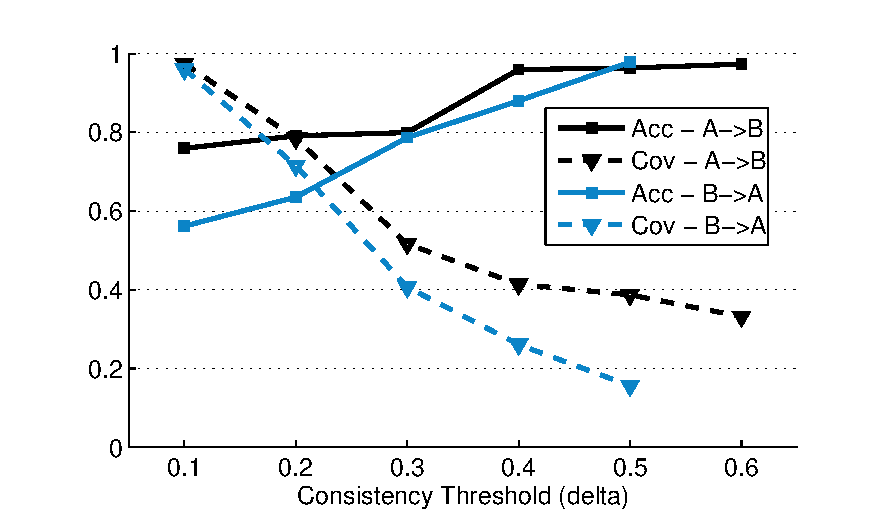
\includegraphics[width=\textwidth]{./fig/TL_AB.eps}
                \caption{A and B}
  \end{subfigure}
  \begin{subfigure}{0.32\textwidth}
                \centering
    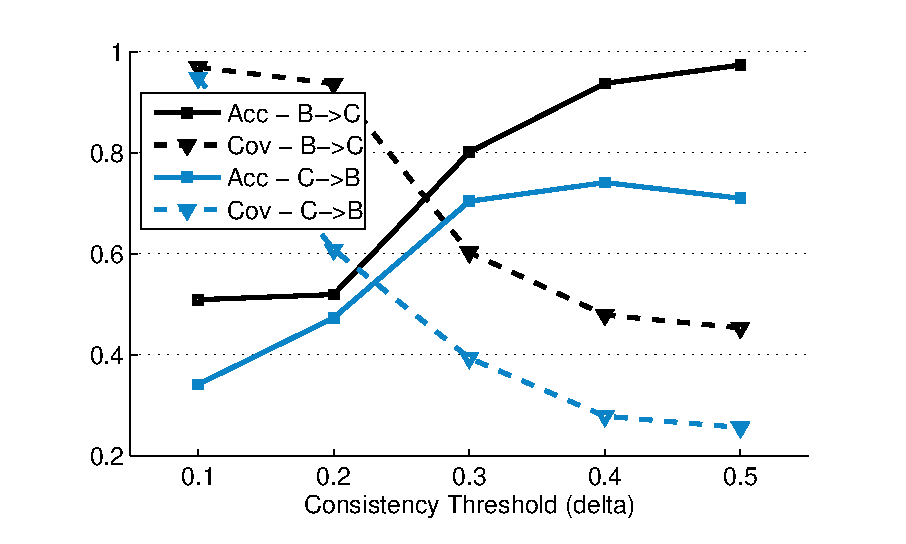
\includegraphics[width=\textwidth]{./fig/TL_BC.eps}
                \caption{B and C}
  \end{subfigure}
  \begin{subfigure}{0.32\textwidth}
                \centering
    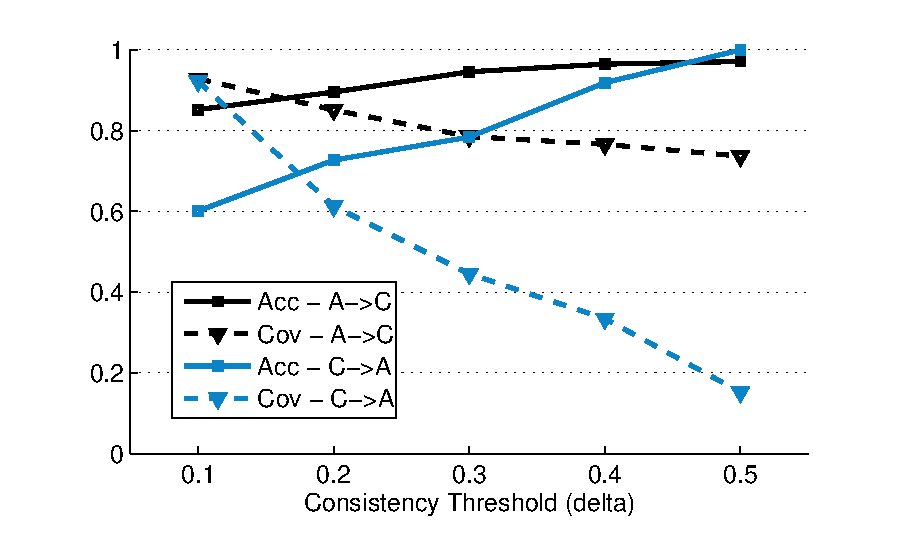
\includegraphics[width=\textwidth]{./fig/TL_AC.eps}
                \caption{A and C}
  \end{subfigure}
\caption{Type classification accuracy (Acc) against labeled percentage (Cov) with transfer learning between different pairs of buildings (denoted as X->Y). As we increase the threshold, the coverage drops while the overall accuracy increases. }
\label{fig:tl_acc}
\end{figure*}

\begin{figure*}[ht!]
\centering
  \begin{subfigure}{0.48\textwidth}
                \centering
    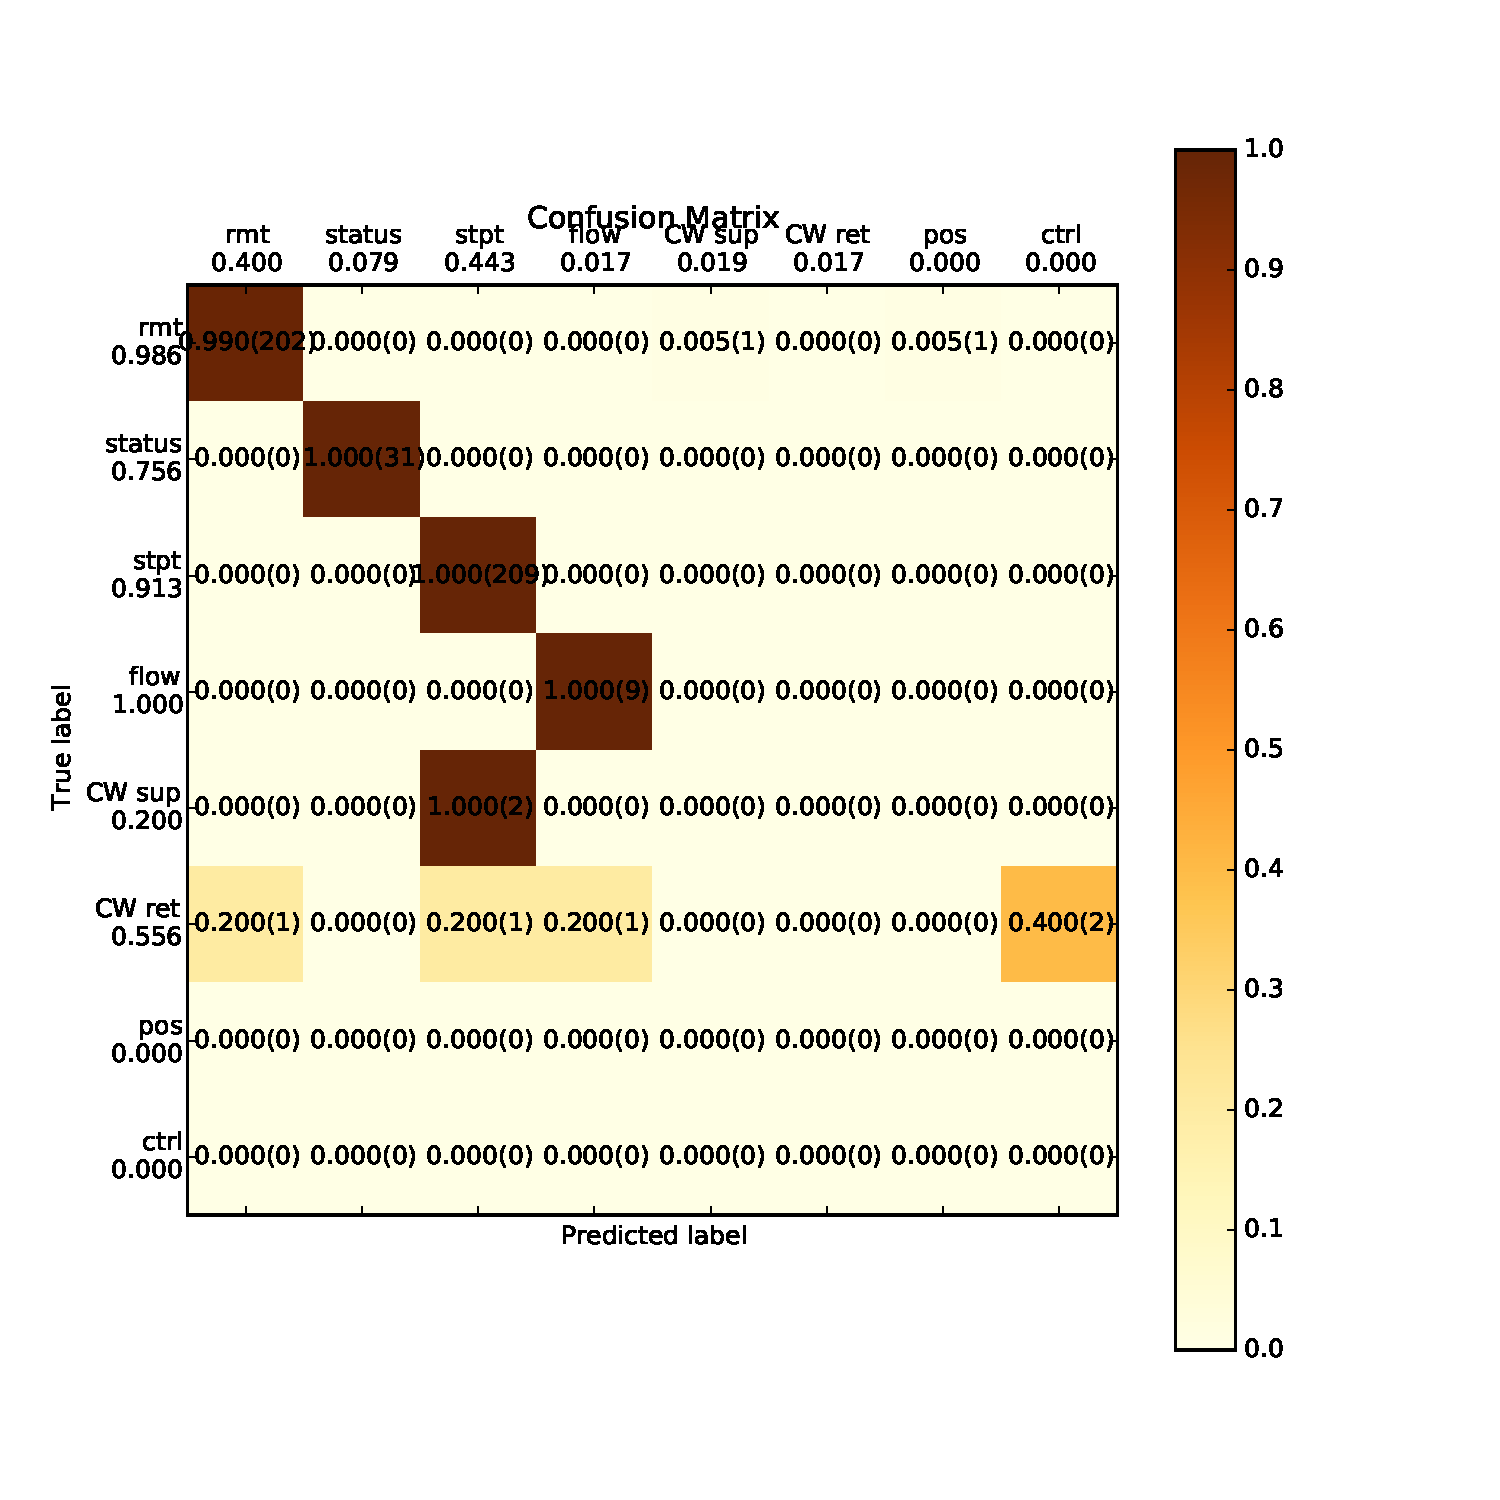
\includegraphics[width=\textwidth]{./fig/cm_multi}
                \caption{Two Sources}
  \end{subfigure}
  \begin{subfigure}{0.48\textwidth}
                \centering
    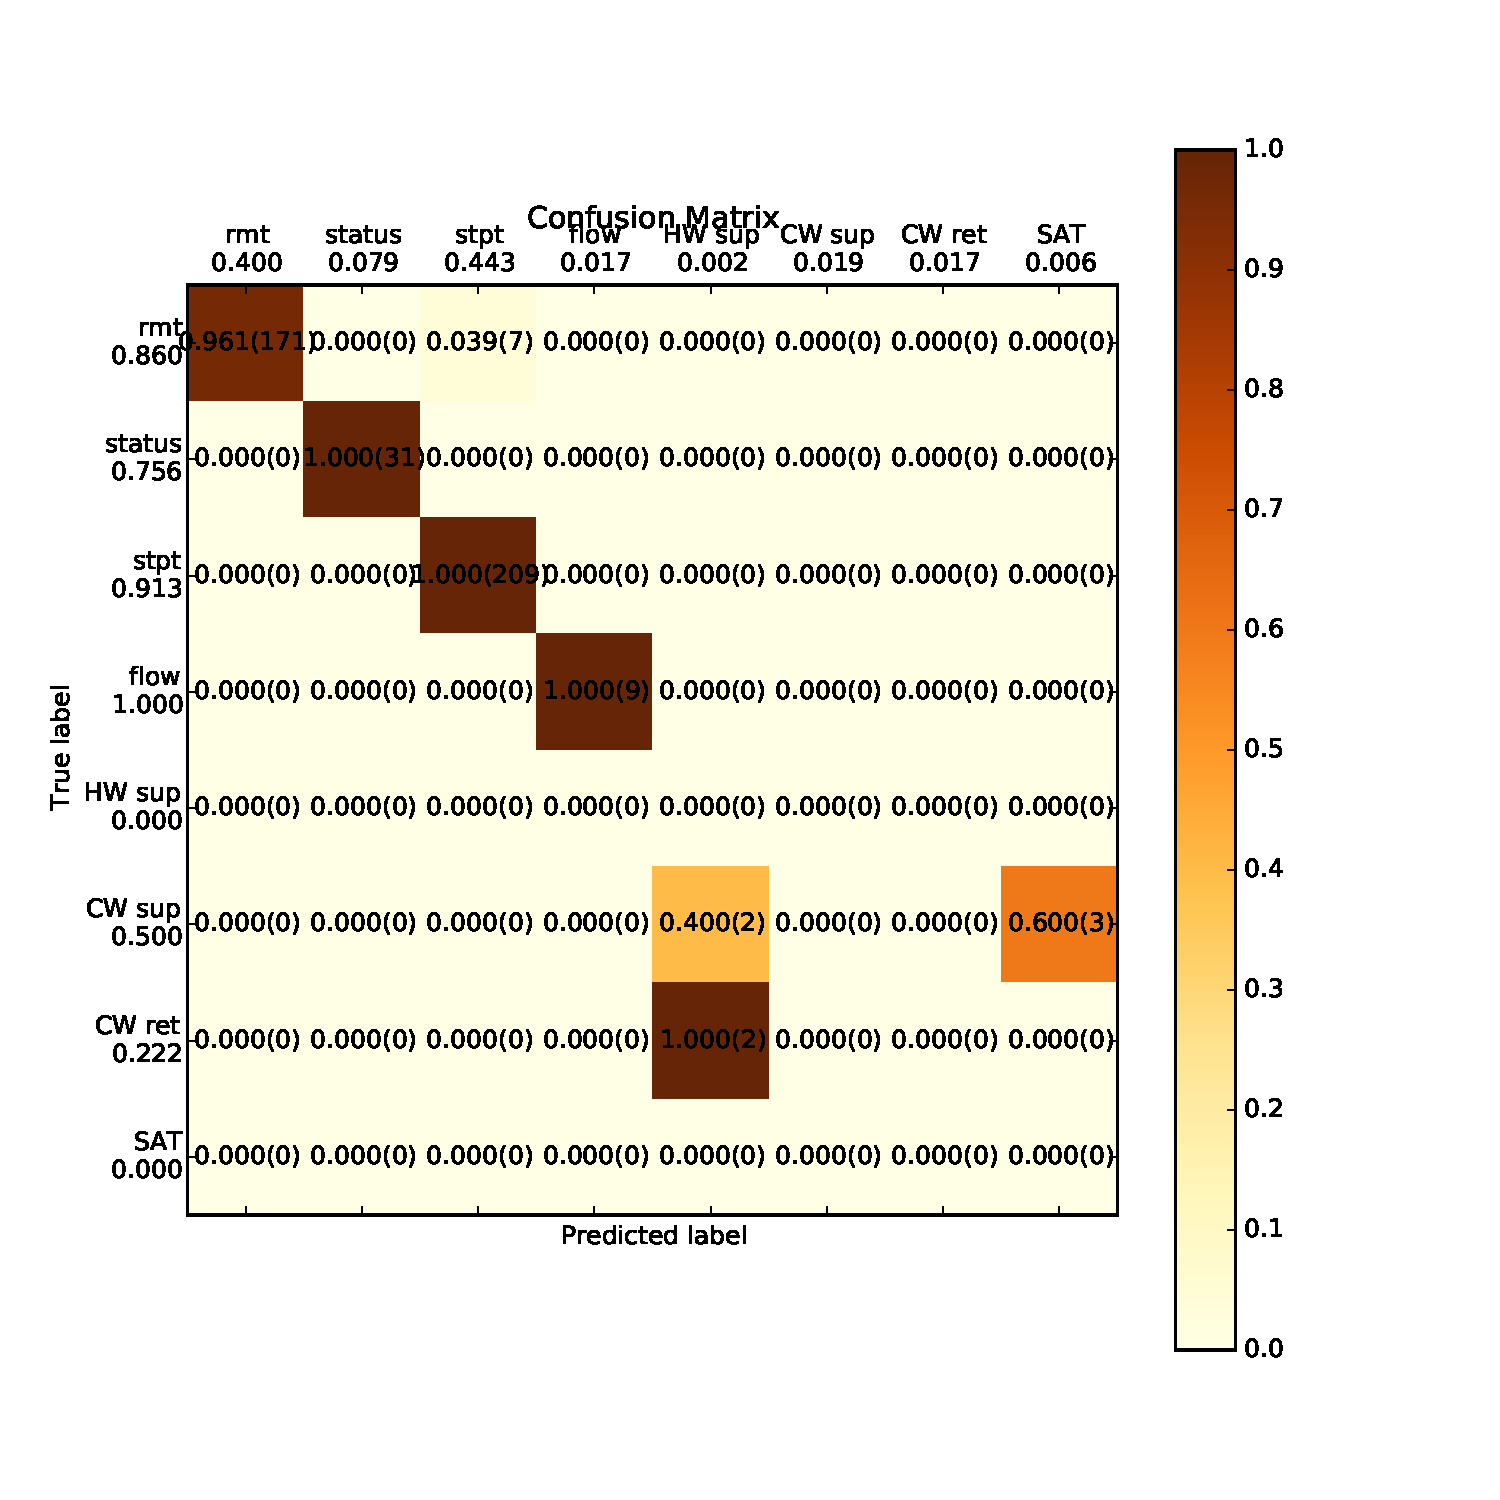
\includegraphics[width=\textwidth]{./fig/cm_single}
                \caption{Single Source}
  \end{subfigure}
\caption{Confusion matrices for the transfer learning classification resuls with two sources and single source: two sources produce higher accuracy by labeling more examples for certain classes. ``rmt'' stands for room temperature, ``stpt'' for setpoint, ``sup'' for supply, ``ret'' for return, ``SAT'' for supply air temperature and ``pos'' for vale position.}
\label{fig_cm}
\end{figure*}


\subsubsection{Base Classifiers and Performance}
\label{sec:baseline}
Our transfer learning based approach employs a few base classifiers. Each base classifier is trained on the same set of data features from the source building. There is no particular requirement on 
what classifiers should be selected in this step.  
We employ three base classifiers: random forest, linear regression (LR) and support vector machines (SVM) with RBF kernels.


\begin{table*}[]
\centering
\begin{tabular}{r|c|c|c|c|c|c}
\hline
\multirow{2}{*}{} & \multicolumn{2}{c|}{Target A} & \multicolumn{2}{c|}{B} & \multicolumn{2}{c}{C} \\ \cline{2-7} 
                  & Acc        & F1        & Acc        & F1        & Acc        & F1        \\ \hline
Source A                 & N/A      & N/A     & 0.943/0.934      & 0.936/0.931     & 0.977/0.970      & 0.981/0.971     \\ \hline
B                 & 0.897/0.875     & 0.932/0.913     & N/A      & N/A     & 0.950/0.952      & 0.939/0.937     \\ \hline
C                 & 0.862/0.862     & 0.864/0.864     & 0.726/0.702      & 0.691/0.726     & N/A     & N/A     \\ \hline
\end{tabular}
\caption{Accuracy and F1 score of transfer learning and the best baseline with $\delta$=0.4. Each cell contains two numbers for our approach and the baseline respectively. Overall, our approach outperforms the baseline.}
\label{table:f1}
\end{table*}

For the three buildings, we have three pairs of choices and for each pair the training/testing can be conducted either way; therefore, we have six testing cases.
The performance of the base classifiers when applied across buildings is shown in Table~\ref{acc_base}.  The base classifiers achieve an accuracy between 0.158 and 0.921.
On average, random forest performs the best, followed by SVM and LR. 
Notice, the accuracy of learning on building C and testing on building B is substantially worse than the other cases. 
One reason is because building B contains many dynamic temperature setpoints whose values change throughout the day, whereas the setpoints in C are static. 
The other type is air flow, whose reading amplitude is significantly different from the ones in C. These two types contribute to most of the errors. %in this case.


\subsubsection{Single Building as the Source}
We first consider the case where only one building is as the source, i.e., each base classifier is trained on data from only one building. 
The overall accuracy of transfer learning for type classification across our three target buildings are illustrated in Figure~\ref{fig:tl_acc}.
There is an intrinsic trade-off between the prediction accuracy and the percentage being labeled, as we set a threshold on the average weight of base classifiers. 
When we increase the threshold $\delta$ on the average weight for base classifiers, we have labels of better quality -- with a drop in the percentage of examples being labeled. 
Empirically, we can set the threshold $\delta$ be around 0.4, which strikes a reasonable balance between accuracy and coverage.

On imbalanced data sets, investigation of accuracy alone is not enough. We also measure the weighted macro F1 score of 
classification for our approach and the baseline. The weighted macro F1 score is an altered version of macro F1 score~\cite{yang}, 
which calculates the F1 score for each class; where ``one-versus-all'' binary classification is performed and weighs the resulting F1 of each class by support (the number of true instances for each label). 

As a baseline, we take the subset of examples in the new building that get labeled by the transfer learning process and apply base classifiers to predict labels on the same population. 
We set $\delta$ to 0.4 and  
repeat 10 times for the experiment in each direction (e.g., A->B). The average of the resuls is reported in Table~\ref{table:f1}. 
Each cell contains two numbers: the former is for our approach while the latter is for the {\it best} baseline.
The case of transferring from C to B is again substantially worse than other cases, this is because the transfer learning algorithm is fundamentally bounded by the performance of base classifiers. 
Intuitively, if none of the base classifiers is able to predict correctly for an instance, no matter how we manipulate the weights, it will not make a difference in the results.
Overall, our approach outperforms the best baseline.
%Paired two sample t-test is performed to validate the statistical significance of improvement from our method over the best-performing baseline. 


\subsubsection{Multiple Buildings as the Source}

\begin{table}[h]
\centering
\begin{tabular}{r|cc|cc}
\hline
\multirow{2}{*}{} & \multicolumn{2}{c|}{Two Sources} & \multicolumn{2}{c}{Single Source} \\ \cline{2-5} 
 & Acc & Cov & Acc & Cov \\ \hline
Target A & {\bf 0.863$^\ast$} & {\bf 0.397$^\ast$} & 0.855 & 0.362 \\ \hline
B & {\bf 0.899$^\ast$} & {\bf 0.458} & 0.874 & 0.455 \\ \hline
C & {\bf 0.980$^\ast$} & {\bf 0.890$^\ast$} & 0.968 & 0.839 \\ \hline
\end{tabular}
\\\noindent
$^\ast p$-value<0.01
\caption{Combining the knowledge from multiple buildings to infer on the new one is superior to exploiting one source building.}
\label{2source}
\end{table}


In practice, it is common to have labels for multiple buildings.  Combining them as a single source should allow us to to achieve better performance.
Using multiple buildings, we repeat the experiments (two ways running for each pair.  We set $\delta$ to 0.4  and use two buildings as the training source. %for the other building. 
From Table~\ref{2source}, we see that combining multiple buildings as the source is superior to single source.  %, as expected.
Figure~\ref{fig_cm} presents the confusion matrices for classification results for the case of using building C as the target.
Two sources achieve a higher accuracy and coverage by correcting some of the errors in room temperature as well as labeling more streams of this type.
Training with data from multiple buildings produces the most robust classifiers and we believe performance improves as you combine data from more
buildings into a single source.
%this rule generalizes to more buildings as the traning source.


\subsection{Complementing Traditional Labeling}
Another important question we want to answer is how much our transfer learning based approach can expedite traditional labeling techniques. 
%Because our method is designed to complement the traditional labeling techniques, rather then replacing them.
A considerable percentage can be automatically labeled by our technique as a first step. The labeling process of a new building can be significantly accelerated.
We adopt the technique developed in~\cite{cikm} and examine how much our technique can accelerate the labeling process.
%~\cite{cikm} formulates a clustering-based active learning approach to iteratively label the type of sensors, where they acquire human label for a ``representative'' example in each iteration and propagate the label to adjacent examples.
For brevity, we refer interested reader to~\cite{cikm} for the detail of the algorithm.

On each testing building, we split the set into 10 folds and run the active learning (AL) and active learning combined with transfer learning (AL+TL), respectively, on nine folds while testing on the remaining one fold.
For the case of AL+TL, we start from the automatic labeling process with a $\delta$ = 0.6 to ensure we have the minimal number of wrong automatic labels. Then we switch to the AL algorithm from~\cite{cikm} where we acquire one manual label per iteration.
We perform 10-fold cross validation for AL and AL+PL and the average of 10 runs are demonstrated in Figure~\ref{fig:comp}. We see that AL+TL help reduce the number of manual labels to achieve the same peformance as AL.
For example, it takes AL+TL 65 iterations to reach 85\% percent while AL takes 80.


\begin{figure}[t]
\centering
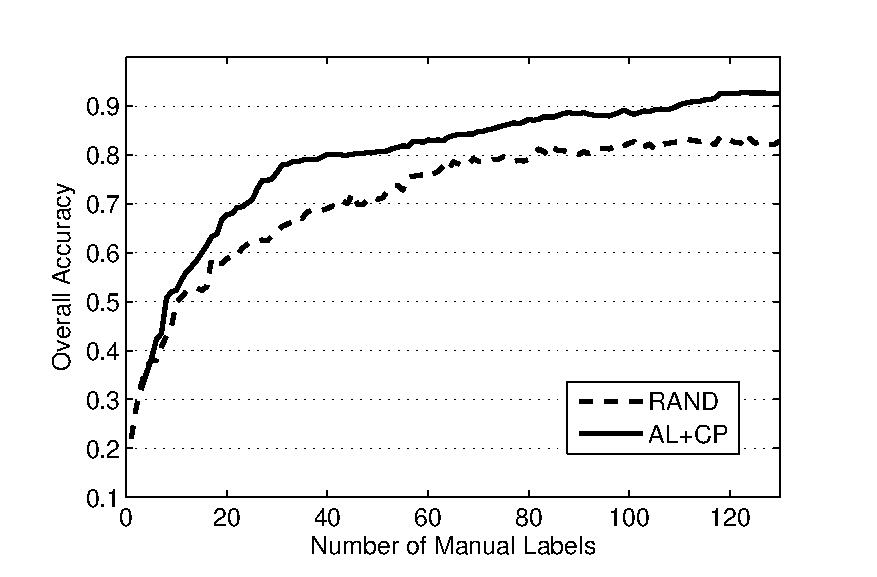
\includegraphics[width=0.4\textwidth]{./fig/tl_al.eps}
\caption{Our transfer learning based approach can complement traditional labeling technique to achieve better acccuracy with the same amount of labels.}
\label{fig:comp}
\end{figure}


\subsection{Discussion}
%\paragraph{Unlabeled Streams}
%With a threshold on the average weight of base classifiers, our transfer learning based technique is able to label a portion of the streams in the new building, which leaves many unlabeled.
%The coverage might be increased by searching for the nearest neighbors in a certain radius to those unlabeled and combine them.
\paragraph{Number of Clusters}
Although we appeal to a non-parametric Bayesion clustering method in our algorithm to generate clusters on the testing building, we further justify such a choice by demonstrating how sensitive the transfer learning can be to the number of clusters generated.

\paragraph{Better Features for Classifiers} The performance of transfer learning and classification processes in our work is bounded by the base classifiers which rely only on a set of general features. The line of work to represent time series with discretized symbols (e.g., the SAX~\cite{sax}) or primitive ``shapes'' (e.g., the ``shapelets''~\cite{shapelet1, shapelet2}) doesn't work well for our problem due to the variability in ``shapes'' and unpredictable ``noises''. We wish to explore how using external or domain-specific knowledge could help improve the classification accuracy. 



%\section{Discussion}
\subsection{Improvement on Classification Accuracy}
We could further explore how using external or domain-specific knowledge would help improve the classification accuracy. For example, if we know the sun sets around 6 PM and observe a trough in the reading of some streams, 

\subsection{Extension of Taxonamy and Class Scope}
We could extend the class scope to include more sensor types because there are more types than the most common ones included in this paper, e.g., alarm sensor, xxx. Meanwhile, we also want to build a more complicated taxonamy for some types, for instance, "setpoints", because there are setpoints for different parameters.  


\section{Conclusion}
We describe a general, simple yet effective transfer learning based approach to accomplish sensor type classification across buildings.
Our technique encapsulates the knowledge from labeled buildings and properly transfer it to other buildings to help the labeling.
By experimenting with over 3000 streams from three buildings on two campuses, our technique is able to automatically label more than xx\% percent of the labels in a new building with at least yy\% accuracy.
We also further demonstrated how much our solution can complement traditional labeling techinique.

Our technique can act as a tool for metadata construction for not only building sensors. 

% is before it becomes a generally viable solution to building metadata construction.


%\section{Acknowledgements}
%Thanks to our shepherd, Kin Cheong Sou, and the anonymous reviewers for helpful comments. Thanks to Albert Goto, for making the first author's stay at UC Berkeley comfortable. Sincere gratitude goes to Kamin and David, for letting this collaboration happen. This work was partly funded by the NSF grants EFRI-1038271 and CPS-1239552.
\bibliographystyle{abbrv}
%\small
\scriptsize
\bibliography{buildsys}

%\balancecolumns
\end{document}
